\documentclass{book}

\usepackage{defs-config-macros}

\begin{document}

\thispagestyle{empty}
\frontmatter
    \begin{minipage}{.3\textwidth}
  \flushleft
  \center{
\includegraphics[scale=.09]{unam.pdf}}

  \vspace{20pt}

  \center{
    \rule{.5pt}{.6\textheight}
    \hspace{7pt}
    \rule{2pt}{.6\textheight}
    \hspace{7pt}
    \rule{.5pt}{.6\textheight}
  } \\

  \center{
\includegraphics[scale=.22]{ciencias.pdf}}
\end{minipage}
\begin{minipage}{.7\textwidth}
\flushright

\center{

  \center{
    \LARGE{U}\large{NIVERSIDAD} \LARGE{N}\large{ACIONAL}
    \LARGE{A}\large{UTÓNOMA} \\[10pt]
    \large{DE}
    \LARGE{M}\large{ÉXICO}
  } \\
  \rule{\textwidth}{2pt}
  \\
  \hrulefill\\[1cm]

  \LARGE{F}\large{ACULTAD DE } \LARGE{C}\large{IENCIAS}\\[2cm]

  \large{
  Análisis del algoritmo \textit{Knuth-Morris-Pratt} con énfasis en la programación funcional
  }\\[1.6cm]

  \huge{
T \hspace{1cm} E \hspace{1cm} S \hspace{1cm} I \hspace{1cm} S  }\\[1cm]

  \large{QUE PARA OBTENER EL TÍTULO DE:}\\[1cm]

  \large{
Licenciado en Ciencias de la Computación  }\\[1cm]

  \large{PRESENTA:}\\[1cm]

  \large{
Ángel Iván Gladín García  }\\[1cm]

  \large{
TUTORA  }\\[.2cm]

  \large{
  Dra. Lourdes Del Carmen González Huesca}\\[1cm]
  \large{
    Ciudad Universitaria, Cd. Mx., 2021
  }
}

\end{minipage}

    \clearpage
    \mbox{}
    \clearpage
    \thispagestyle{empty}
    
    \pagenumbering{Roman} 


\begin{center}
{\Large \textbf{Hoja de Datos del Jurado}}
\vspace*{.85cm}
\end{center}


\begin{enumerate}

\item Datos del Alumno

Gladín \\
García \\
Ángel Iván \\
+52 55 8196 8560 \\
Universidad Nacional Autónoma de México \\
Facultad de Ciencias \\
Ciencias de la Computación \\
313112470


\item Datos de la Tutora

Dra. \\
Lourdes del Carmen \\
González \\
Huesca


\item Datos del Sinodal 1

Dr. \\
Favio Ezequiel \\
Miranda \\
Perea


\item Datos del Sinodal 2

Dra. \\
Adriana \\
Ramírez \\
Vigueras


\item Datos del Sinodal 3

Dr. \\
Canek \\
Peláez \\
Valdés


\item Datos del Sinodal 4

L. en C.C. \\
Fernando Abigail \\
Galicia \\
Mendoza


\item Datos del trabajo escrito

{\small Análisis del algoritmo \textit{Knuth-Morris-Pratt} con énfasis en la programación funcional} \\
100p. \\ % TODO: cambiar el número de hojas
2021 


\end{enumerate} 

    
    \chapter*{Agradecimientos}
    \lipsum[1-2]

    \clearpage
    
    \tableofcontents

\mainmatter
    \chapter*{Motivación y estructura del trabajo}
        En mi camino aprendiendo y escribiendo programas usando programación funcional, es algo común ver un programa
que aunque sea corto y legible, muchas veces es algo ineficiente. Entonces es ahí cuando Richard Bird tiene
en mente que un programa debe actuar como la especificación formal del problema, pero también por medio del
razonamiento ecuacional poder calcular uno más eficiente.
Uno de los factores que ayudó al crecimiento en el interés de la programación funcional, fue que en los años
1990's se dieron cuenta que estos lenguajes son buenos para hacer razonamiento ecuacional.
De hecho el lenguaje funcional Gofer, inventado por Mark Jones capturó este pensamiento como un acrónimo 
(\textit{Good for equational reasoning}).
\newline

Lo que se abordará en este trabajo es primero empezar con una especificación en Haskell y después proseguir a
calcular una versión más eficiente por medio de razonamiento ecuacional.
La razón de este trabajo es ver hasta donde el diseño de un algoritmo puede estar encajado en una forma
matemática de calcular un resultando usando principios matemáticos bien establedicos como definiciones, 
teoremas, y \textit{``leyes''}.
Curiosamente, es generalmente verdadero que en matemáticas los cálculos están diseñados para simplificar
cosas complicadas, en el diseño de algoritmos usualmente es al revés.
\begin{quote}
Simples, pero ineficientes programas son transformados en versiones más eficientes que puedes ser
completamente opacas en su implementación.
\end{quote}
Explicando las ideas detrás de un algoritmo es mucho más fácil en un estilo funcional, en vez de un
procedimental. Las funciones pueden ser separadas fácilemente, cada una es sucinta y capturan patrones
de cómputo.
\newline

Los algoritmos de búsqueda de subcadenas (\textit{String Matching Algorithms}) son usados frecuentemente en:
programas de edición de texto para encontrar todas las ocurrencias de un patrón en un texto, para encontrar
patrones particulares en una cadenas de ADN, o también en algunos motores de búsqueda los utilizan para
encontrar páginas web en búsquedas, entre otras aplicaciones. Algoritmos efecientes para atacar este tipo de
problemas nos ayudan gratamente para mejorar el tiempo de la búsqueda.
\newline

TODO

Como lo menciona Richard S. Bird en su artículo \emph{Polymorphic String Matching}\cite{book:1505279}
% TODO: ponerle un formato bonito
El desarrollo de cálculos en programas funcionales ha sido asociado a trucos de magia: agradables de ver pero seguido pero a menudo hay un misterio en cómo se hacen.

En este trabajo se explicará esto, es dar un cálculo del algoritmo KMP,
%FIXME: quitar lo de abajo?
Este probleme de string matching está formulado polimórficamente, así que la única propiedad disponible que tienen los elementos del alfabeto es que sean comparables.

% TODO: de aquí me puedo sacar algunas ideas
% https://www.cs.princeton.edu/~rs/AlgsDS07/21PatternMatching.pdf

    \addcontentsline{toc}{chapter}{Motivación y estructura del trabajo}
    
    \chapter{Fundamentos}
        \section{Programación funcional}
\subsection{Definiciones inductivas y recursivas}

\section{Listas}
\section{Definiciones de listas}
\subsection{Inducción sobre listas}
\section{\textit{Tupling}}

\section{Pliegues}
\subsection{\texttt{foldr}}
\subsection{\texttt{foldl}}
\subsection{Propiedad Universal}
\subsection{Principio de fusión}
\subsection{\textit{Scan Lemma}}\label{fundamentos:scan_lemma}
En esta sección se considerará la función \hsCode{scanl}, \hsCode{scanl} aplica un pliegue
izquierdo (\hsCode{foldl f e}) a cada segmento (todos los prefijos) de una lista como se muestra
a continuación,

\begin{minted}{haskell}
scanl (@) e [x, y, z, ...] = [e, e@x,(e@x)@y,((e@x)@y)@z,...]
\end{minted}

Se propondrá la siguiente especificación de \hsCode{scanl} como:
\begin{minted}{haskell}
scanl :: (b -> a -> b) -> b -> [a] -> [b]
scanl f e = map (foldl f e) . inits

inits :: [a] -> [[a]]
inits []     = [[]]
inits (x:xs) = [] : map (x:) (inits xs)
\end{minted}

Ejemplo:
\begin{minted}{haskell}
>>> scanl (+) 0 [1..10]
[0,1,3,6,10,15,21,28,36,45,55]
\end{minted}

La expresión anterior calcula la suma de cada prefijo de una lista de números del 1 al 10.
\begin{minted}{haskell}
[0, 0+1, (0+1)+2, ((0+1)+2)+3, (((0+1)+2)+3)+4, ...]
\end{minted}

Veamos un ejemplo de \hsCode{scanl}
\begin{minted}{haskell}
>>> inits [1..5]
[[],[1],[1,2],[1,2,3],[1,2,3,4],[1,2,3,4,5]]
\end{minted}

Pero se puede ver que la definición propuesta de \hsCode{scanl} involucra evaluar \hsCode{f} un
total de $\sum_{i=0}^{n} i = \frac{n(n+1)}{2}$ veces sobre una lista de longitud $n$.

Es aquí cuando uno se pregunta si ¿se podría hacer mejor?. La respuesta es sí, cálculando una mejor
definiciónpor medio de razonamiento ecuacional. Cosideremos por casos.

\begin{itemize}
\item Caso \hsCode{[]}
\begin{minted}{haskell}
scanl f e []
  = -- {Definición de scanl}
map (foldl f e) (inits [])
  = -- {Por inits.1}
map (foldl f e) [[]]
  = -- {Por map.1 y map.2}
(foldl f e []) : map (foldl f e) []
  = -- {Por foldl.1 y map.1}
e : []
  = -- {Azucar sintáctica}
[e]
\end{minted}

Teniendo así que \hsCode{scanl f e [] = [e]}.

\item Caso \hsCode{x:xs}
\begin{minted}{haskell}
scanl f e (x:xs)
  = -- {Definición de scanl}
map (foldl f e) (inits (x:xs))
  = -- {Por inits.2}
map (foldl f e) ([] : map (x:) (inits xs))
  = -- {Por map.1 y map.2}
(foldl f e []) : (map (foldl f e . (x:)) (inits xs))
  = -- {Por foldl.1}
e : (map (foldl f e . (x:)) (inits xs))
  = -- {Por la afrimación que se demostrará abajo y que es el caso (x:xs)}
e : map (foldl f (f e x)) (inits xs)
  = -- {Por la primera definición de scanl.1}
e:scanl f (f e x)
\end{minted}

\textbf{Afirmación:} \hsCode{foldl f e . (x:) = foldl f (f e x)}. Se seguirá como una consecuencia
inmediata de \hsCode{foldl}.

\begin{itemize}
\item Caso \hsCode{x:[]}
\begin{minted}{haskell}
foldl f e . (x:) []
  = -- {Composición de funciones}
foldl f e [x]
  = -- {Aplicación y azucar sintáctica}
foldl f (f e x) []
  = -- {Por foldl.1 y Por foldl.2}
e
\end{minted}

\item Caso \hsCode{x:ys}, análogo al anterior.
\end{itemize}
\end{itemize}

Teniendo así una nueva definición de \hsCode{scanl} como,
\begin{minted}{haskell}
scanl f e []     = [e]
scanl f e (x:xs) = e:scanl f (f e x) xs
\end{minted}

donde \hsCode{f} solo se calcula un número lineal de veces, a diferencia de su primera definición
propuesta que requería un número cuadrático de veces.

Aunque si vemos definición\footnote{
\url{https://hackage.haskell.org/package/base-4.14.1.0/docs/src/GHC.List.html\#scanl}
} del preludio es diferente:
\begin{minted}{haskell}
scanl                   :: (b -> a -> b) -> b -> [a] -> [b]
scanl                   = scanlGo
  where
    scanlGo           :: (b -> a -> b) -> b -> [a] -> [b]
    scanlGo f q ls    = q : (case ls of
                               []   -> []
                               x:xs -> scanlGo f (f q x) xs)
\end{minted}

Pero esto de debe a que la versión que se calculó da \hsCode{scanl f e undefined = undefined} y la
versión de preludio \hsCode{scanl f e undefined = e:undefined}. Esto se debe a que como Haskell
es perezoso, no nos debemos de preguntar nada acerca de la lista a procesar, pero lo que es seguro
es que empieza con \texttt{e}.

En general, cualquier problema que involucre la función \hsCode{inits}, este lema es bastante útil
de saber porque si recordamos la primera especificación:
\begin{minted}{haskell}
scanl f e = map (foldl f e) . inits
\end{minted}

La LHS toma $\Theta(n)$ el número de evaluaciones de \hsCode{f} mientras que RHS toma $\Theta(n^2)$.
Y como se demostró ambas expresiones son equivalentes.

\begin{figure}[h]
\caption{Un ejemplo concreto de la versión propuesta inicialmente de \texttt{scanl} y la que se derivó}
\centering
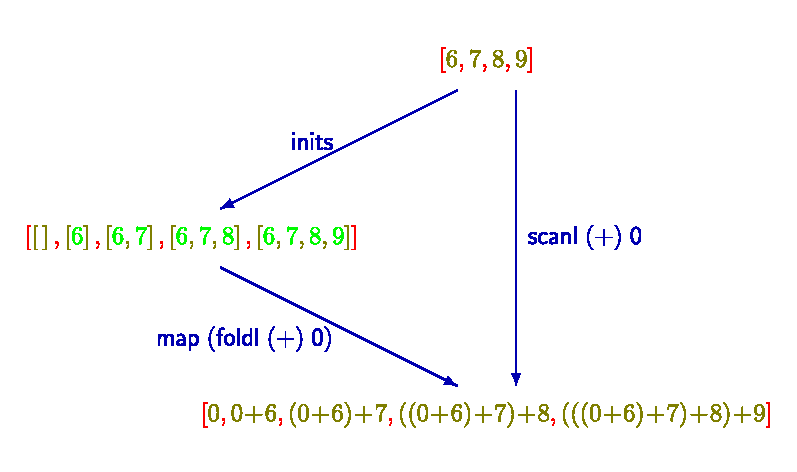
\includegraphics[width=0.9\textwidth]{scan_lemma_example.pdf}
\end{figure}

\subsection{\textit{The maximum segment sum}}

\section{Razonamiento ecuacional}

\section{Definiciones de funciones}

\section{\textit{Strict property}}



% Parece ya estar listo
\section{Analizando el tiempo}
\subsection{Notación asintótica}
\subsection{Estimando tiempo}
\subsection{Tiempo amortizado}
\subsection{Algunos ejemplos} % TODO: aquí hacer énfasis en la prog funcional

% Esta sección ya está lista
\section{Cadenas}
\subsection{Notación y terminología}
Decimos que el patrón $P$ \textbf{ocurre con un desplazamiento} $s$ en el texto $T$ si
$0 \leq s \leq n - m$ y $T[s+1 \ldots s+m] = P[1 \ldots m]$. Si $P$ ocurre con un desplazamiento
$s$ en $T$, entonces se dice que $s$ es \textbf{un desplazamiento válido}, si no, se dice que $s$
es \textbf{un desplazamiento inválido}.
El \textbf{problema de búsqueda de subcadenas} es el problema de encontrar todos los
desplazamientos válidos en los que dado el patrón $P$ ocurre en el ttexto $T$.
% aquí poner la imagen del la figura 32.1 y explicarlo

\subsection{String matching} % TODO: ver si dejarlo o cambiarlo al español
En diversas situaciones se necesita encontrar todas las ocurrencias de un patrón en un texto;
éstas pueden ir desde editores de texto hasta buscar patrones particulares en secuencias de ADN.
Es aquí cuando se hace uso de algoritmos eficientes para este problema.

Es aquí cuando se formaliza el problema de ``búsqueda de subcadenas'' (string-matching).
Supongamos que el texto es un arreglo $T[1 \ldots n]$ de longitud $n$ y el patrón es un arreglo
$P[1 \ldots m]$ de longitud $m \leq n$. También supongamos que los elementos de $P$ y $T$ son
caracteres tomados de un alfabeto finito $\Sigma$. El arreglo de caracteres $P$ y $T$ también son
llamados \textbf{cadenas} de caracteres.



Denotemos a $\Sigma^*$ como el conjunto de todas las cadenas de longitud finita formadas usando
caracteres del alfabeto $\Sigma$. La cadena de longitud cero es \textbf{la cadena vacía}, denotada
como $\varepsilon$, que también pertenece a $\Sigma^*$. La longitud de una cadena $x$ se denota
como $\vert x \vert$. La \textbf{concatenación} de dos cadenas $x$ y $y$, se denota como $xy$ y
tiene como longitud $\vert x \vert + \vert y \vert$ y consiste de los caracteres de $x$ seguidos
por los caracteres de $y$.

Decimos que una cadena $w$ es \textbf{prefijo} de una cadena $x$, denotada como $w \sqsubset x$, si
$x = wy$ para alguna cadena $y \in \Sigma^*$. Notemos que si $w \sqsubset x$, entonces
$\vert w \vert \leq \vert x \vert$. De manera análoga, decimos que una cadena $w$ es \textbf{sufijo}
de una cadena $x$, denotado como $w \sqsupset x$, si $x = yw$ para alguna $y \in \Sigma^*$. Y así
como con el prefijo, si $w \sqsubset x$, entonces $\vert w \vert \leq \vert x \vert$.
Por ejemplo, tomemos \texttt{ab $\sqsubset$ abcca} y \texttt{cca $\sqsupset$ abcca}. La cadena
vacía $\varepsilon$ es tanto un sufijo coomo un prefijo para cualquier cadena.

\subsection{Algunos algoritmos comunes de búsqueda de subcadenas}

\subsection{Problemas} % TODO: ver si dejo esto aquí lo muevo y cambiar el título

\begin{tcolorbox}
  \hypertarget{repetition_factor}{32.1 a.}
  \textbf{String matching based on repetition factors}
  Let $y^i$ denote the concatenation of string y with itself $i$ times. For example,
  \texttt{ab}$^3 =$ \texttt{ababab}. We say that a string $x \in \Sigma^*$
  \textbf{has repetition factor} $r$ if $x = y^r$ for some string $y \in \Sigma^*$ and some $r > 0$.
  Let $\rho(x)$ denote the largest $r$ such that $x$ has repetition factor $r$.
  Give an efficient algorithm that takes as input a pattern $P[1 \ldots m]$ and computes the value
  $\rho(x)$ for $i = 1,2,\ldots,m$. What is the running time of your algorithm?
  \end{tcolorbox}
  
  Lo primero que se debe de hacer es calcular la función de error $\pi$ teniendo una complejidad en
  tiempo de $\Theta(m)$ y lineal en espacio. Teniendo calculada $\pi$, consideremos $m$ la longitud
  del patrón y supongamos que $r = m - \pi[m]$ es la longitud de la $i$-esima raíz del patrón y que
  $\pi[i] = i - r$ donde $r \mid m$ es la $\frac{i}{k}$-ésima concatenación de la raíz del patrón
  hasta la $i$-ésima posición. Conlcuyendo así que $\rho(P) = \frac{m}{r}$.
  
  En otro caso, supongamos que no se cumple lo anterior, i.e., que $r \nmid m$ entonces su factor de
  repetición forzosamente debe ser 1. Por contradicción, supongamos que tiene un factor de repetición
  mayor estrico que 1 lo que significaría que tendría que habría una cadena $y^r$ y que
  $\pi[i] \geq \vert x^{r-1} \vert$, pero significaría que podríamos escribir a $x$ concatenada $r$
  veces. $\Rightarrow\!\Leftarrow$.
  
  
  \begin{tcolorbox}
  \hypertarget{cyclic_rotation}{32.4-7}   
  Give a linear-time algorithm to determine whether a text $T$ is a cyclic rotation of another string
  $T'$ . For example, \texttt{arc} and \texttt{car} are cyclic rotations of each other.
  \end{tcolorbox}
  
  Descartemos el caso en que la longitud de $T$ y $T'$ sean diferentes porque no podría ser una
  rotación cíclica. Entonces $\vert T \vert = \vert T' \vert$, sea $S = TT$ el texto donde $T$ está
  concatenado dos veces, y $P = T'$ el patrón. Usando el algoritmo de Knuth-Morris-Pratt se buscará
  el patrón $P$ en $S$ en tiempo lineal.
  
  Supongamos que $P$ aparece en $T$ desplazado $s$ posiciones a la izquierda donde
  $0 \leq s < \vert P \vert$. Si $s = 0$ entonces $T = T'$, el caso interesante es cuando $s > 0$,
  teniendo así que $T[0 \ldots s]$ es sufijo de $T'$ y $T[s+1 \ldots m]$ es prefijo de $T$. 
  
  \noindent\rule{\textwidth}{1pt}
  
  Los problemas anteriores se obtuvieron del libro \textit{Introduction to Algorithms, Third
  Edition}\cite{cormen_2009}, pero en el \autoref{chap:jueces} se verá que éstos mismos problemas
  pueden llegar a aparecer en problemas de programación competitiva, por lo que no basta con
  ``memorizar los algoritmos'' como muchos podrían llegar a pensar.
  

% Misc que tal vez podríia utilizar
% TODO: aquí agarrar cosas del polymorphic en la parte que dice: on compositioin https://wiki.haskell.org/Tutorials/Programming_Haskell/String_IO
% TODO: https://www.khanacademy.org/computing/computer-science/algorithms/asymptotic-notation/a/asymptotic-notation
    
    \chapter{Búsqueda de subcadenas con perspectiva en \\la programación imperativa}
    \chaptermark{} % https://tex.stackexchange.com/questions/26234/chapter-title-in-header-too-long
        \section{Algoritmo de búsqueda de subcadenas ingenuo (\textit{naïve})}

\begin{algorithm}[H]
    \SetKwProg{Fn}{NAIVE-STRING-MATCHER($T,P$)}{}{}
    \Fn{}{
        $n = T.length$\\
        $m = T.length$\\
        \For{$s = 0 $ \KwTo $n-m$}{
            \If{$P[1\ldots m] == T[s+1 \ldots s+m]$}{
                $print$ ``Pattern occurs with shift'' $s$
            }
        }
    }
\end{algorithm}

\section{Función de error}
\label{imperativo:pi} % TODO: aquí poner lo de los saltos

\section{De Morris-Pratt a Knuth-Morris-Pratt}
% TODO: https://www.cs.helsinki.fi/u/tpkarkka/teach/14-15/SPA/lecture04.pdf
% https://studylib.net/doc/7580926/chapter-6-the-mp-and-kmp-algorithms--algorithms-based-upon

% http://www-igm.univ-mlv.fr/~lecroq/string/node7.html#SECTION0070
%http://www-igm.univ-mlv.fr/~lecroq/string/node8.html
% DEL LIBRO DE STRINGOLOGY SACAR ALGO

\section{Knuth-Morris-Pratt}
% TODO: ver qué agarro de aquí: https://en.wikipedia.org/wiki/Knuth%E2%80%93Morris%E2%80%93Pratt_algorithm


\begin{algorithm}[H]
    \SetKwProg{Fn}{KMP-MATCHER($T,P$)}{}{}
    \Fn{}{
        $n = T.length$\\
        $m = T.length$\\
        $\pi =$ COMPUTE-PREFIX-FUNCTION($P$)\\
        $q = 0$\\    
        \For{$i = 1 $ \KwTo $n$}{
            \While{$q >0$ and $P[q+1] \neq T[i]$}{
                $q = \pi[q]$
            }
            \If{$P[q+1] == T[i]$}{
                $q = q + 1$
            }
            \If{$q == m$}{
                $print$ ``Pattern occurs with shift'' $i-m$\\
                $q = \pi[q]$
            }
        }
    }
\end{algorithm}

\begin{algorithm}[H]
    \SetKwProg{Fn}{COMPUTE-PREFIX-FUNCTION($P$)}{}{}
    \Fn{}{
        $m = P.length$\\
        let $\pi[1 \ldots m]$ be a new array\\
        $\pi[1] =0$\\
        $k = 0$\\    
        \For{$q = 2 $ \KwTo $m$}{
            \While{$k >0$ and $P[k+1] \neq P[q]$}{
                $k = \pi[k]$
            }
            \If{$P[k+1] == P[q]$}{
                $k = k + 1$
            }
            $\pi[k] = k$
        }
        \Return $\pi$
    }
\end{algorithm}

\section{Implementación en C++}
\inputminted{cpp}{codigo/cpp/kmp.hpp}

    
    \chapter{Búsqueda de subcadenas con perspectiva en \\la programación funcional}
    \chaptermark{} % https://tex.stackexchange.com/questions/26234/chapter-title-in-header-too-long
        % TODO: introducción-

\section{Función de error}
En esta seccióno se derivará por medio de una especificación formal la función de error del
algoritmo de KMP. Aunque por medio de este acercamiento\cite{bird:cyclic} se podría obtener todo
el algoritmo KMP usando estructuras cíclicas (específicamente listas doblemente ligadas) no se
hará así, porque se verá otra manera más ``elegante'' de hacerlo en la siguiente sección.

Consideremos la cadena \texttt{abacabab} y su procesamiento con la función de error,

\begin{table}[h]
\centering
\begin{tabular}{c|c|c|c|c|c|c|c|c|}
\cline{2-9}
$k$      & 1          & 2          & 3          & 4          & 5          & 6          & 7          & 8          \\ \hline
$P[k]$   & \texttt{a} & \texttt{b} & \texttt{a} & \texttt{c} & \texttt{a} & \texttt{b} & \texttt{a} & \texttt{b} \\ \hline
$\pi[k]$ & 0          & 0          & 1          & 0          & 1          & 2          & 3          & 2          \\ \cline{2-9} 
\end{tabular}
\end{table}

\begin{center}
La entrada $\pi[k]$ es la longitud del \textbf{sufijo propio más largo} de
\hsCode{take k xs} que también es un prefijo de\hsCode{ xs}.
\end{center}

Veamos el procesamiento de la cadena de arriba:
\begin{itemize}
\item[$\pi{[1]}$] Dado que el sufijo propio más largo de \hsCode{take 1 xs} para
cualquier\hsCode{ xs} no vacía siempre es $\varepsilon$, siempre se tendrá que $\pi[1] = 0$.
\item[$\pi{[2]}$] El sufijo propio más largo de \hsCode{take 2 "abacabab" = "ab"} que también es
prefijo de \texttt{abacabab} es $\varepsilon$. Por lo que $\pi[2] = 0$.
\item[$\pi{[3]}$] El sufijo propio más largo de \hsCode{take 3 "abacabab" = "aba"} que también es
prefijo de \texttt{abacabab} es \texttt{a}. Por lo que $\pi[3] = 1$.
\item[$\pi{[4]}$] El sufijo propio más largo de \hsCode{take 4 "abacabab" = "abac"} que también es
prefijo de \texttt{abacabab} es $\varepsilon$. Por lo que $\pi[4] = 0$.
\item[$\pi{[5]}$] El sufijo propio más largo de \hsCode{take 5 "abacabab" = "abaca"} que también
es prefijo de \texttt{abacabab} es \texttt{a}. Por lo que $\pi[5] = 1$.
\item[$\pi{[6]}$] El sufijo propio más largo de \hsCode{take 6 "abacabab" = "abacab"} que también
es prefijo de \texttt{abacabab} es \texttt{ab}. Por lo que $\pi[6] = 2$.
\item[$\pi{[7]}$] El sufijo propio más largo de \hsCode{take 7 "abacabab" = "abacaba"} que también
es prefijo de \texttt{abacabab} es \texttt{aba}. Por lo que $\pi[7] = 3$.
\item[$\pi{[8]}$] El sufijo propio más largo de \hsCode{take 8 "abacabab" = "abacabab"} que también
es prefijo de \texttt{abacabab} es \texttt{ab}. Por lo que $\pi[8] = 2$.
\end{itemize}

Para una lista \textbf{no vacía} \texttt{as} los sufijos \textbf{propios} de \hsCode{take k as},
son sufijos de \hsCode{take (k - 1) (tail as)}. El $k-1$ es porque como se afirma que la lista
\texttt{as} es no vacía, se contempla a la lista vacía en la lista de sufijos propios, y a
\hsCode{tail as} porque por definición de sufijo \textbf{propio} no puede estar la cabeza de
la lista \texttt{as}.

Teniendo así una forma de calcular todos los sufijos \textbf{propios} de una lista \texttt{as} como:
\begin{minted}{haskell}
[take (k - 1) (tail as) | k <- [1 .. length as]] = inits (tail as)
\end{minted}
donde \hsCode{inits}\footnote{
    La función \hsCode{inits} viene definida en el módulo \hsCode{Data.List}.
} regresa una lista con los prefijos de una lista en orden creciente y \hsCode{tail} extrae la
cabeza de la lista.

Ejemplo con \texttt{abacabab}:
\begin{minted}{haskell}
>>> inits (tail "abacabab")
    inits "bacabab"
    ["","b","ba","bac","baca","bacab","bacaba","bacabab"]
\end{minted}

La función de error se define como:
\inputminted[fontsize=\small, frame=single, framesep=10pt]{haskell}
    {codigo/haskell/FailureFunctionNaive.hs}

Donde \hsCode{llsap as bs} (\textit{\textbf{L}ength of \textbf{L}ongest \textbf{S}uffix of
\texttt{bs} that is \textbf{A}lso a \textbf{P}refix of \texttt{as}}) es la longitud del sufijo más
largo de \texttt{bs} que es también un prefijo de \texttt{as}. La función \hsCode{llasp} primero
\hsCode{tails}\footnote{
    La función \hsCode{tails} viene definida en el módulo \hsCode{Data.List}.
} regresa todos los sufijos en orden decreciente y con \hsCode{isPrefixOf} solo toma el los sufijos
que son prefijos de \texttt{as}. Finalmente con la función \hsCode{head} se obtiene el primero
elemento que evidentemente es el mayor.

Se hace un sínonimo para el tipo \hsCode{[(Int, (a, Int))]} con la palabra reservada \hsCode{type}
llamado \hsCode{PiTable} para mayor legibilidad. La primera entrada es la $i$-ésima posición del
elemento y en la segunda entrada es una tupla, corresponde a la función dee error.

Y así \hsCode{ptable} calcula la función de error como una lista de \hsCode{PiTable}.

Si se calcula \hsCode{ptable "abacabab"} el resultado es:
\begin{minted}{haskell}
>>> ptable "abacabab"
    [(1,('a',0)),(2,('b',0)),(3,('a',1)),(4,('c',0)),(5,('a',1)),
     (6,('b',2)),(7,('a',3)),(8,('b',2))]
\end{minted}

Recordando el \textit{Scan Lemma}\ref{fundamentos:scan_lemma}, que afirma que
\begin{minted}{haskell}
map (foldl op e) . inits = scanl op e
\end{minted}

y viendo que hay un \hsCode{inits} en la definición de \hsCode{ptable} en\\
\hsCode{map (llsap as) (inits (tail as))} veamos como lo podemos utilizar. Pero problema aquí es
que \hsCode{llasp as} debe ser expresado como una instancía de \hsCode{foldl (op as) e}. Ahora se
debe mostrar que:

\begin{minted}{haskell}
llsap as []          = e
llsap as (bs ++ [b]) = op as (llsap as bs) b
\end{minted}
Para una definición adecuada de \hsCode{e} y \hsCode{op}. 

Es inmediato que \hsCode{llsap as [] = 0} porque el sufijo \texttt{[]} (que es el más largo) que
es prefijo de \texttt{as} es de longitud 0 y así \texttt{e = 0}. De hecho este caso es el primer
elemento de \hsCode{inits (tails as)}.

Lo interesante aquí es encontrar \hsCode{op}. Supongamos\hsCode{ k = llsap as bs} donde \texttt{k}
es la longitud del sufijo más largo de \texttt{bs} que es un prefijo de \texttt{as} y,
\hsCode{ a = head (drop k as)} donde \texttt{a} es el siguiente elemento de \texttt{as} después
del prefijo más largo de \texttt{as} que se empareja con el sufijo de \texttt{bs}.

Para ejemplificarlo consideremos los siguientes ejemplos sobre la cadena \texttt{abacabab}.
\begin{itemize}
\item Consideremos\hsCode{ bs = "ba"} donde\hsCode{ k = llsap "abacabab" "ba" = 1} y así\\
\hsCode{ a = head (drop 1 "abacabab") = head "bacabab" = 'b'}.\\
Quedando \texttt{a\colorbox{yellow}b}\texttt{acabab}.
\item Consideremos\hsCode{ bs = "bacab"} donde\hsCode{ k = llsap "abacabab" "bacab" = 2} y\\
así\hsCode{ a = head (drop 2 "abacabab") = head "acabab" = 'a'}.\\
Quedando \texttt{ab\colorbox{yellow}a}\texttt{cabab}.
\end{itemize}

Si \texttt{a = b}, entonces \hsCode{llsap as (bs ++ [b]) = k + 1} porque cuando se esté
``consumiendo'' \texttt{b}, significa que el prefijo de \texttt{as} ya en el paso anterior ya era
un sufijo de un segmento de \texttt{bs}, y así solamente lo que se tenía de longitud más larga del
prefijo en el paso pasado solo se suma uno.
% TODO: poner aquí un ejemplo

En otro caso significa que hasta el $i$-ésimo caracter consumido no ha habido ningún sufijo que sea
prefijo de y así \texttt{k = 0} entonces \hsCode{llsap as (bs ++ [b]) = 0}.

Quedando este último caso,
\begin{minted}{haskell}
llsap as (bs ++ [b]) = llsap as (take (k - 1) (tail as) ++ [b])
\end{minted}
este caso parece que no decir mucha información, pero es justamente cuando % TODO: poner referencia a la versión impetattiva cuando se regresa a buscar otra entrada en pi[i]
% TODO: poner referencia al capitulo donde pongo el código impertaivo y como "se va saltando"


Para mostrar este caso consideremos el siguiente ejemplo: % TODO: mejorar este esbozo de ejemplo
\begin{itemize}
\item \hsCode{as = "abacabab"} \hsCode{bs = "bacabab"}\\
\hsCode{llsap as (bs ++ [b]) = llsap as (take (k - 1) (tail as) ++ [b])}\\ % 
\hsCode{llsap "abacabab" ("acabab" ++ "b") = 3 = llsap as ((take 2 "abacabab") ++ "b")}
\hsCode{llsap "abacabab" ((take 2 "abacabab") ++ [b]) = llsap "abacabab" ("ab" ++ "b")}
\end{itemize}

Así \hsCode{llasp as bs = foldl (op as) bs}, donde
\begin{minted}{haskell}
op as k b  | a == b    = k + 1
           | k == 0    = 0
           | otherwise = llsap as (take (k - 1) (tail as) ++ [b])
               where a = head (drop k as)
\end{minted}

Aún no se ha acado de razonar el programa. Haciendo la siguiente observación,
\begin{minted}{haskell}
llsap as (take (k - 1) (tail as) ++ [b]) = op as (llsap as (take (k - 1) (tail as))) b
\end{minted}
% TODO: explicar que es porque se consume la b, o sea el primer elementos de la lista bs, pero se ocupa la función op


En Haskell existe un módulo de arreglos %TODO: poner aquí todo eso
% TODO: mejorar explicación culera
y se usará para acceder a la $k$-ésima posición en la lista 
y así para acceder como

% TODO: decir que aquí usaré ya arrays
\begin{minted}{haskell}
head (drop k as)                            = fst (xs ! (k + 1))      -- (ec.1)
op as (llsap as (take (k - 1) (tail as))) b = op as (snd (xs ! k)) b  -- (ec.2)
\end{minted}

% TODO: revisar si lo que escribí hace sentido.
\begin{itemize}
\item En \texttt{(ec.1)} como se quiere acceder al siguiente elemento en la lista \texttt{xs} para
obtener \texttt{a}, primero se obtiene la posición $k+1$ de la lista y despues con \hsCode{fst}
se obtiene el tipo \hsCode{a}. % TODO: ver como se llama 'a' formalmente.
\item En \texttt{(ec.2)} La \hsCode{(snd (xs ! k))} es el más largo y se obtiene de lo que se había
procesado anteriormente.
% TODO: Explicar mejor
\end{itemize}

\newpage

Finalmente usando Arreglos %TODO: explicar mejor
la versión final queda como.
\inputminted[fontsize=\small, frame=single, framesep=10pt]{haskell}
    {codigo/haskell/FailureFunctionOptimized.hs}
% TODO: poner una conclusión
\newpage

\section{Knuth-Morris-Pratt}

    \chapter{\textit{QuickCheck}}
        \epigraph{\itshape Randomized testing exemplifies the 80/20 rule: it yields 80\% of the benefit
of formal verification for 20\% of the effort.}{Matt Might}

\QuickCheck es una biblioteca de Haskell para hacer pruebas generadas aleatoriamente que deben
cumplir ciertas propiedades nuestros programas. El programador provee una especificación de su
programa en la forma de propiedades las cuales las funciones deben satisfacer y, \QuickCheck prueba
que esas propiedades se mantengan en un gran número de casos de casos generados aleatoriamente. Las
especificaciones son expresadas en Haskell usando combinadores proporcionados por \QuickCheck.
\QuickCheck provee combinadores para definir propiedades, observar la disctribución de los casos
de prueba y, definir los generadores de información generadores.\footnote{
    Descripción de \QuickCheck tomada de la documentación oficial\\
    \url{https://hackage.haskell.org/package/QuickCheck}.
}

\noindent\rule{\textwidth}{1pt}

En esta sección se verá la importancia sobre usar \QuickCheck; tanto como una manera rápida de
verificar ciertas propiedades que deben cumplirse en alguna implementación que se haya hecho en
Haskell, ventajas y desventajas sobre su uso. El porqué es útil utilizarlo y qué problemática
aborda.

Se verá como será utilizado en un ejemplo práctico; en este caso tanto en
\hyperlink{funcional:funcion_error}{la funsión de error} y en
\hyperlink{funcional:kmp}{\textit{Knuth-Morris-Pratt}} en Haskell. En ambos ejemplos se expondrá la
versión \textit{naïve} y la versión ``optimizada'' que fue derivada mediante razonamiento
ecuacional. Y por medio de casos generados aleatoriamente se analizará el resultado que
\QuickCheck proporciona.

\section{Motivación}
Hoy en día el estilo de hacer pruebas a nuestro código es mediante \textit{pruebas unitarias (unit
testing)} en las cuales; se inveta un ``estado del mundo'', se ejecuta la prueba unitaria, se
checa si el estado modificado del ``mundo'' hace lo que debería hacer y al final se ve si todo
sigue funcionando como se debe.

A continuación se muestra un conjunto de aserciones (\texttt{assert}) en Java para ejemplificar
la idea. Una aserción puede ser utilizada para verificar si una suposición hecha durante la
implementación del programa se mántiene válida cuando el programa es ejecutado.

\begin{minted}[frame=lines, framesep=10pt, linenos]{java}
public class TestAdder {
    public void testSum() {
        Adder adder = new AdderImpl();
        assert(adder.add(1, 1) == 2);
        assert(adder.add(1, 2) == 3);
        assert(adder.add(2, 2) == 4);
        assert(adder.add(0, 0) == 0);
        assert(adder.add(-1, -2) == -3);
        assert(adder.add(-1, 1) == 0);
        assert(adder.add(1234, 988) == 2222);
    }
}

interface Adder {
    int add(int a, int b);
}
class AdderImpl implements Adder {
    public int add(int a, int b) {
        return a + b;
    }
}
\end{minted}

En este tipo de pruebas se pueden agregar gran cantidad de objetos que simulan comporamientos 
(\textit{mock objects}) o, un sinnúmero de casos prueba pero ¿cuál es el problema aquí? El código
anterior solo tiene 7 pruebas y no es dificil de imaginar que se pueden crear muchos más casos, o
simplemente si se implementa otra funcionalidad el espacio de búsqueda de posibles \textit{bugs}
crece de forma exponencial.

Claramente hacer pruebas es impráctico, pero ¿por qué usar \QuickCheck?
\begin{itemize}
\item Se pueden combinar las pruebas basadas en propiedades (en la siguiente sección se hablará
de esto) con casos de prueba generados \textit{aleatoriamente}.
\item El programador escribe propiedades a cumplir en vez de pruebas en específico.
\item Obviamente no nos puede dar la misma seguridad de hacer pruebas exhaustivamente, pero
\textbf{es muy práctico}.
\item Se puede escoger la cantidad de información que será sometida a nuestras propiedades.
\end{itemize}


\section{Uso básico}

Consideremos la siguiente propiedad de la función \hsCode{reverse} para \textit{listas finitas}.
\begin{minted}{haskell}
import Test.QuickCheck

prop_rev_rev :: [Int] -> Bool
prop_rev_rev xs = reverse (reverse xs) == xs
\end{minted}

Después de haber importado \hsCode{Test.QuickCheck}, se carga la definición en \texttt{ghci}
para después invocarlas
\begin{minted}{text}
>>> quickCheck prop_rev_rev
+++ OK, passed 100 tests.
\end{minted}

Y aunque esta propiedad es verdadera y más adelante se muestra su demostración, se puede
ver lo útil y práctico que es.
% TODO: Poner prueba de StructuralInduction.pdf página 9

Ahora consideremos un caso donde la propiedad falle \QuickCheck mostrará un contraejemplo.
\begin{minted}{haskell}
prop_wrong :: [Int] -> Bool
prop_wrong xs = reverse xs == xs 
\end{minted}

Mostrando así un caso donde no cumple la propiedad.
\begin{minted}{text}
>>> quickCheck prop_rev_id
*** Failed! Falsified (after 5 tests and 3 shrinks):
[1,0]
\end{minted}

\noindent\rule{\textwidth}{1pt}

Veamos otro ejemplo, para todo entero $n$, si $n$ es par entonces $n+1$ es impar. Aunque la
demostracióon es trivial, con \QuickCheck se puede validar (mas no verficar formalmente) con
varios números generados aleatoriamente para probar esta propiedad.
\begin{minted}{haskell}
>>> quickCheck (\n -> even n ==> odd(n + 1))
+++ OK, passed 100 tests
\end{minted}

donde \hsCode{==>} es una propiedad condicional que descarta los casos que no satisfacen esa
precondición.

Cuando se escriben propiedades;
\begin{itemize}
\item Las propiedades simples son función que son funciones booleanas.
\item La conveción es que los nombres de las propiedades tienen el prefijo \hsCode{prop_}.
\item Los parámetros están ímplicitamente cuantificados con un cuantificador universal $\forall$ y
la última y más importante es que las funciones polimórficas deben de estar restringidas a un tipo
en específico.
\end{itemize}


\section{Generadores}

Aunque \QuickCheck puede generar algunos valores aleatorios para algún tipo ímplicitamente, hay
ocaciones que se necesita nuestros propios valores aleatorios. Es aquí cuando se debe escribir
una instancia de \hsCode{Arbitrary} para esto. Los valores que se ocupan en la pruebas son
producidos por los \textit{generadores de valores}.

Los Generadores tienen tipos de la forma \hsCode{Gen a} que es un generador de valores para
un tipo \hsCode{a}. El tipo \hsCode{Gen} es una mónada, así que se puede utilizar la notación 
\hsCode{do} y las funciones monádicas pueden ser utilizadas para definir generadores.

Veamos el siguiente ejemplo; consideremos el tipo de dato algebraico \hsCode{Point} donde
representa un punto en un espacio bidimensional. Lo que se quiera hacer es generar puntos
con coordenadas $x$ y $y$ aleatoriamente.

\begin{minted}{haskell}
data Point = Point Int Int

instance Arbitrary Point where
  arbitrary = do
    x <- arbitrary
    y <- arbitrary
    return (Point x y)
\end{minted}

donde \hsCode{arbitrary :: Gen a} es un generator para valores de un cierto tipo, y que en este
caso son de tipo \hsCode{Int}.

\section{Probando las implementaciones}

Es aquí cuando las versiones \emph{naïve} y las obtenidadas por medio de razonamiento ecuacional,
tanto en la \hyperlink{funcional:funcion_error}{función de error} como en
\hyperlink{funcional:kmp}{\textit{Knuth-Morris-Pratt}} son probadas uno a uno con diferentes casos
prueba en Haskell.

Al hacer los casos prueba usando el tipo \hsCode{String} es poco probables tener
\textit{una buena disctribución} de los caracteres que comprende la cadena y, en especial en probar
el algoritmo KMP con las cadenas del patrón y texto. Si por ejemplo restringimos las cadenas
a que solo contengan caracteres ASCII aún así no serían muy útiles en las pruebas. Consideremos
el siguiente ejemplo.

\begin{minted}{haskell}
>>> sample $ vectorOf 10 arbitraryASCIIChar
\end{minted}
La función \hsCode{sample :: Show a => Gen a -> IO ()} genera algunos valores de ejemplo y los
imprime en la slaida estándar. Si se toma un valor que se imprimió que por ejemplo sería
\mintinline{text}|"\t\n]*]i_\fm\SYN"| se ve que no es muy útil para nuestro propósito. Pero
¿no sería más mejor definir nuestros propios valores aleatorios?

\hfill \break
En los generadores presentados a continuación en la función de error y el algoritmo KMP es
bastante usual que se trabaje sobre alfabeto finito $\Sigma$; puede ser sobre las letras del
alfabeto $\Sigma = \{ \texttt{a} \ldots \texttt{z} \}$, un alfabeto binario $\Sigma = \{ 0, 1 \}$
o un alfabeto de ADN donde $\Sigma = \{ \texttt{A,C,G,T} \}$.

\newpage
\inputminted[frame=lines, framesep=10pt, linenos]{haskell}
    {codigo/haskell/test-failure-function.hs}

\begin{itemize}
\item En la línea \texttt{3} y \texttt{4} se importan los módulo de la versión de error, tanto
la versión que tiene complejidad $O(n^3)$ y $\Theta(n)$ respectivamente que proveerán la función
\hsCode{ptable} que es la función de error.
\item En la línea \texttt{6} del módulo \hsCode{Data.Array} solo se importa la función\\
\hsCode{elems :: Array i e -> [e]} para obtener una lista de elementos del arreglos en el orden
indexado.
\item En la línea \texttt{8} se hace una envoltura (\emph{wrapper}) para un \hsCode{String} con el
constructor \hsCode{S}. Éste será usado para poder usar la instancia de \hsCode{Arbitrary}.

Mucho mejor definir un nuevo tipo isomorfo a (en este caso) \hsCode{String} y así poder definir
su generador por defecto para éste para usos específicos.
\item En la línea \texttt{11} a \texttt{15}, para poder usar \hsCode{arbitrary} es el tipo
\hsCode{Pattern} definido por nosotros, se necesita declar como instancia de \hsCode{Arbitrary}.
En la línea \texttt{12} por medio de la notación \hsCode{do} cada línea será un valor monádico,
primero se liga el valor \hsCode{size} a un número aleatorio entre 1 y 1000 con\\
\hsCode{chooseInt :: (Int, Int) -> Gen Int} que genera un elemento aleatorio dado un rango
inclusivo, acto seguido se liga la variable \hsCode{text} con una cadea del tamaño de la variable
\hsCode{size} sobre un alfabeto de la letra \hsCode{'a'} a la \hsCode{'z'} con
\hsCode{vectorOf :: Int -> Gen a -> Gen [a]} que genera una lista de una longitud dada. Finalmente
con la función \hsCode{return} pone el resultado en un contexto monádico.
\item En la línea \texttt{17} no es necesario que sea instancia de \hsCode{Show}, pero con
\hsCode{verboseCheck} en \hsCode{QuickCheck} es útil para poder mostar los casos prueba.
\item De la línea \texttt{22} y \texttt{24}
% TODO: explicarlo propiamente que es eso de que requresa bool y lo que saco del constructor
% poner como se llama lo que hace let e iin
en la línea se transforma lo que devuelve la función \hsCode{ptable} a una lista de tipo
\hsCode{[(Char, Int)]} donde la $i$-ésima posición donde la primera entrada es el $i$-ésimo caracter
de la cadena de  y la segunda entrada es la $i$-ésima posiición de la función de error.
En la línea \texttt{23}, lo que regresa \hsCode{FailureFunctionOptimizedp.ptable} regresa
\hsCode{Array Int (a, Int)} pero con la función \hsCode{A.elems} se obtiene un lista que finalmente
en la línea \texttt{24} see compara que ambas listas sean iguales.
\end{itemize}

% TODO: ver si ocupo esto: \hsCode{elements :: [a] -> Gen a} Genera un elemento de los valores dados. La lista debe ser no vacía.

\texttt{\$ runhaskell test-matching.hs}

\begin{minted}{text}
Testing NaiveMatching with MP1...
+++ OK, passed 100 tests.
Testing MP1 with MP2...
+++ OK, passed 100 tests.
Testing MP2 with KMP...
+++ OK, passed 100 tests.
Testing NaiveMatching with KMP...
+++ OK, passed 100 tests.
\end{minted}

\begin{minted}{text}
Passed:
jwvtllqfgknosijmqccjmpwrfjjbaxgqakfhkxvhwjgukoeoipneicodymknicywsrwjwiz
rzoeufakcwyojquaugelxiujdbrexedtmsqhoofquvrucbvvwmjpbeeamiajfrrruvwjixl
pvrrntqyxyopxyoynhpghrknnrikcukgyjamnngkytmqmdmydzqeendgktbltsfdqwhjfhn
cnroyrelnsskwereataldovaxpneqmvnjaxengwvlknppfzrlmvpyeatvhvbatesajcfpcf
upltdezxedaggbhavklpiyjzwk

Passed:
ovfpnmsesopulhcnpjzhsubeuwfsrvcrktozf

Passed:
lgcnmiwzyvtlkpsuukuemwawrdptrulmchwmtqkknymyfnyurmobjhgkpcfrxbxfxhjerks
mehenlcjjwbbkzhxdotgxwasmxgwpmsnhlsoyfshqclxscaxytdwywxozhvqpbkshf

Passed:
wmdtscgkwkkuuxwqmmvdexwvtdplthvgtjbcacxmnncqlnzhfnskrfaynnvcogyqllfkzcc
gwtuyjxlstlrvphafeajgjwwahyqnqgfutvtsfqeqiulljouzkjgvtwgrrnhfpznugyawox
ypqwiubmkylfhrwnbdfkhbnnqpnrmebivpbypkswtnrrmitdgxwqjmfoetqhwuqbbghvmko
wscxbzdl

Passed:
ruhtwpwesozzglmsvzzshonujhutwjkagfhzbdvsdiczpeuzxgwmkugjgpbynlp

...
...
...

+++ OK, passed 100 tests.

\end{minted}

% TODO: poner que cambié a verboseCheck

% TODO: acabar el ejemplo de abajo
\newpage
\inputminted[frame=lines, framesep=10pt, linenos]{haskell}
    {codigo/haskell/test-matching.hs}
\begin{itemize}
\item En la línea \texttt{3}, \texttt{4}, \texttt{5} y \texttt{6}
\item En la línea \texttt{8}
\item En la línea \texttt{11}
\item En la línea \texttt{19}
\item foo %TODO: poner en todos los "prop"
\end{itemize}

\begin{minted}{text}
Testing NaiveMatching with MP1...
Passed:
Pattern:GCCGAACCATCGAGTGTATC
Text:TAAGACAATTCAACTCCGAGCTGCGCGGCGCAGTTTGTCACAGTGTGGGGGTGGCAGCTACCCCCTAAG
CGTTATTTATTGGTGTACGCTGAGTATCACAATATTCCACCACCCTCCGTTATGGTTAGTTGATAGAAATTCGA
CCGATGTTTGATTCTTCTAAAGCCAGTGTAACTGCGGATAAGCTGGCTTGG

Passed:
Pattern:CCA
Text:TGCATTAGCGGGTGAGGAGCTCTACGCTTCGCTTTCAGCTTTAAACGATTATGTGCGGTCACCCCAATT
GTCTTATGATGGCCAATATTTCGTCAGTACCACTTCAGTGGCATGACTGAGTGACGCA

Passed:
Pattern:C
Text:CACCACGCCGATTCCTGGTCGTTACCTTAGCCAAATAGACTTAAGTGTTGCTTGACCTGTC

Passed:
Pattern:CGTTGTG
Text:GGGTATCATGACTCCGAAGGATTTGTGACGTTGTGAGGATTTACACCCCGTGAGTCGATCTTTCCTGGT
CTTGATGATGAGATGCGGCACGAAGGTAGGGACTACTTAAGAGGGTCGCTCAAGTAGGATCTGGACGTGTACAG
ACTATCACACCTCTCGCGCCGTACTACTGTTAATCCCCTCTCTCTTGCCATCTGAGCTAGCGCTCAGCTCGATA
TTTGTTTTATA

Passed:
Pattern:AG
Text:AAAAGCGGAACTCAATCTGCCAAGCGCCCGAGCACCTGTGGCCTCGCACTGTGGTGGCGAAGTGTTAAG
GCATGAACCTTATGCCGTAGCAACTTGCACACATACTTTGCATCTAACCTCCACTTAATCCGCGGCGATTGCAT

...
...
...

+++ OK, passed 100 tests.

Testing MP1 with MP2...
Passed:
Pattern:TACGCTTCCGCCTCGTAT
Text:GGTTGCTACACCCCGTCTGCCACCGATACATGGTAGCACTACTTAGCTATGGAGTCCGAAAGAAACCAG
GTATCCGGTAGAATGGATTTAGCGAGGTAATAGGGTCCAGCTTTCAAGCTCAACCCATC

Passed:
Pattern:AGG
Text:CCCGGCTATTGTCCCAAAGCATGATCATAACTTCAAGCTGTGTCCCCTTCTCAGTCGGACAGCGCTAGA
ATCCGCCCGTAGGCAGAACGAAGTGATCGATTTACAGTGTTTTGAAAAGGCCGTCCTGAAACACGCGTCTGTTA
TGTAATTGTGGTATCTTCTACTAGATTTGTGTCATCA

...
...
...

+++ OK, passed 100 tests.

Testing MP2 with KMP...
Passed:
Pattern:CCC
Text:CCTCGACAACAGGTATTCAAGTGTGCATCCATCTTATAGAAGTACATTCAATAACCGTCTAAGCTGCTG

Passed:
Pattern:CGG
Text:AGGCCAGAGCCATTGAACTGAAGAAATAAAGCGTGGCACGACGCACCACCTGCCGCATCTCTCGGCGCA
CACGTTGTGTCTGTGTCCGGTAAAAAATACATATAATCCATACATGTT

...
...
...

+++ OK, passed 100 tests.

Testing NaiveMatching with KMP...
Passed:
Pattern:CCGCATCTGGAGTGG
Text:TCCTGACGGATGAATAGTCTGCCCGACGATTCTTGCTTGACTGCTTATGGTGGTACACTCGTAGAGGGT
GGGGACGTGCTTCAGACCTTAACAGCTTATCGTCTCTGTGTGAACGGTACACGCGACGATACATCGTCCGTAGG
ATTTGCACGGGCGTTCCGCATCTGGAGTGGCTAGATTCAGTTGTAA

Passed:
Pattern:TCA
Text:TCGGAAGGCGACGAGTGCGATAAGAGTCAGCAATAGTTGTGCCTAAGCCATATGATGCCAGACCGCCGTCATCACTCTCGTAGTCAGGCACTTGAGCTTAAGGTTATCAATTTATCGGGTATTTTTGACATGGCAGGTAAGGGGGATCGCTTTAGCATGTTAGTAACCCGAAAGACATGATTTTGACATCTCACACGTAGTTATGGAAGCAACTGCCCTACGGCTCCAGGCGAGCCAACTGCGCCTAGTGGGTGTGCCTGCGCTTAACGACCACTGATTGGTTAGTCTGATCCACGAGGGCGGCCAAGGACAAGCATAGACCTGGGCCCCCCTCGGTGCGGCACTAAGATATATCCTGATGGACCACCGATATTTTAATGTGGGCACCTACAGGATTCATATGTCAATTATACGATAGATAAAGGATGACCGGGACACACATCGA

...
...
...

+++ OK, passed 100 tests.
\end{minted}

% TODO: revisar si lo que escribí hace sentido.

    \chapter{Jueces en línea}
        \label{chap:jueces}

En esta sección se resolverán 2 problemas relacionados con \textit{string matching} usando el
algoritmo KMP y la función de error de la que se habló en el capítulo 4. Se resolverán los
problemas usando C++ y Haskell y se compararán ambas versiones.

Es un estándar que las especifiaciones del problema estén en inglés.

%% TODO: Explicar los constraints

\section{SPOJ}
SPOJ (Sphere Online Judge)
% https://wiki.haskell.org/SPOJ
% Tomar algo del competitive aquí

\section{Problemas}

% TODO: poner aquí la motivación.

\subsection{Encontrar el factor de repetición de una cadena}
Recordemos en el \hyperlink{repetition_factor}{capítulo 3 el problema 32.1}, es aquí cuando lo
bonito de la programación competitiva y resolver ejercicios teóricamente se juntan. Ése problema
es lo mismo a resolver el siguiente, y aún mejor, en un juez en línea que puede ``probar'' la
implementación considerando ciertas restricciones.

La especificación del problema dice lo siguiente: 

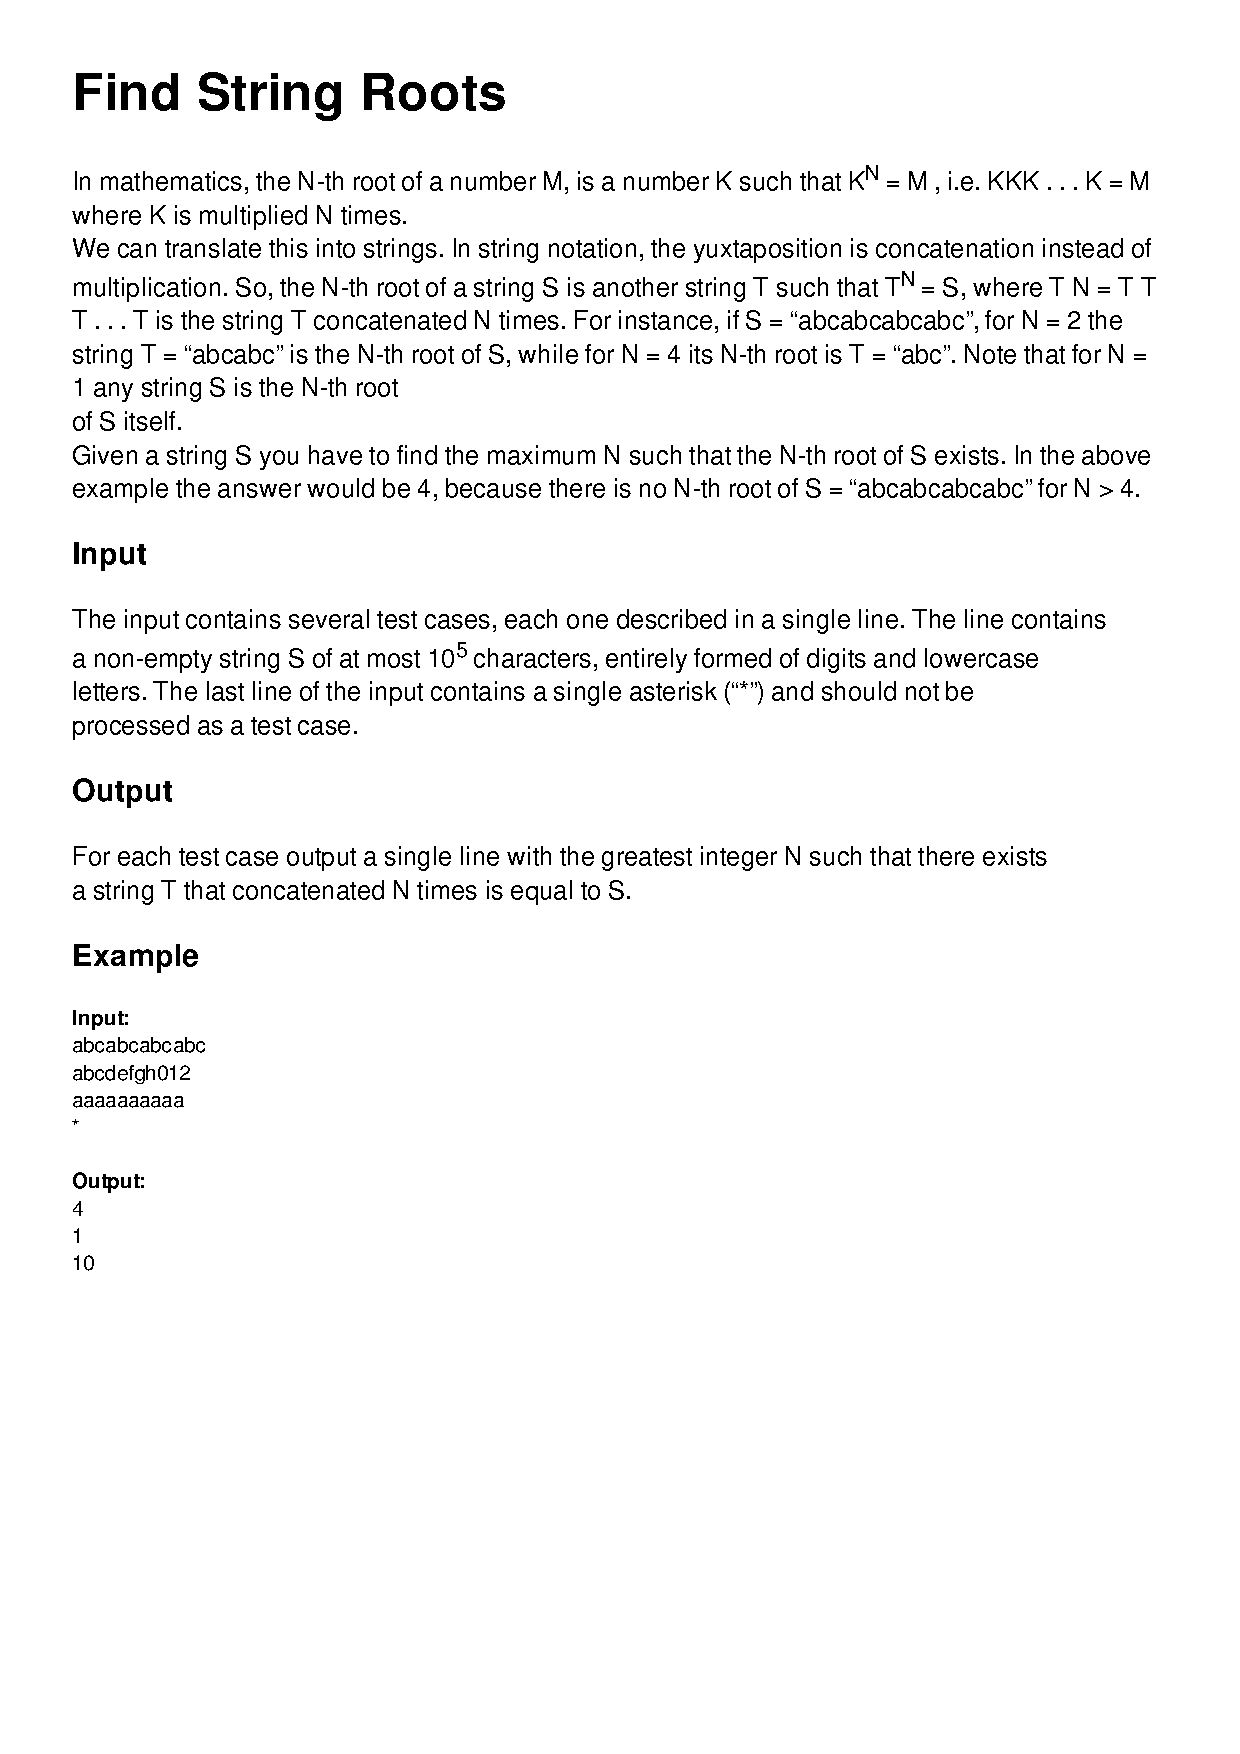
\includepdf[pages=-]{problemas/pdf/FINDSR.pdf}

\subsubsection{Análisis}
Como se había dicho previamente, ya se había atacado este problema así que se omitirá el análisis
y la complejidad.

\subsubsection{Entrada}
Una \textit{heurística} a seguir es que siempre que diga: \textit{``the input contains several test
cases, each line described in a single line''} es leer hasta el final de archivo (End Of File) cada
línea. Seguido de esto, dice que cada línea una cadena no vacía de a lo más $10^5$
caracteres\footnote{Hay lenguajes programación que no tienen implementadas cadenas, y que se debe
saber de antemano el tamaño, para así tener un arreglo de $n$ caracteres. Es aquí cuando es
importante saber el tamaño máximo de la entrada.} formada solamente de dígitos y letras en
minúsculas\footnote{También es sumamente importante saber si las cadenas del lenguaje que se usará
como son represntadas ya que podrían estar en ASCII o Unicode.}.
Finalmente dice que la última entrada contiene un solo asterisco \texttt{*} y que no debe ser
procesado como un caso más.

\subsubsection{Salida}
Para cada caso prueba \textit{(input)} se debe imprimir en la salida estándar una sola línea con un
número $n$ siendo ésta la raíz de la cadena, es decir, el número de veces que está concatenada la
cadena consigo misma.

\subsubsection{Ejemplos}
\begin{itemize}
\item Consideremos la entrada $x =$ \texttt{abcabcabcabc} y sobre ésta se construye la función
de error, 
\begin{table}[h]
\centering
\begin{tabular}{c|c|c|c|c|c|c|c|c|c|c|c|c|}
\cline{2-13}
$i$      & 1          & 2          & 3          & 4          & 5          & 6          & 7          & 8          & 9          & 10         & 11         & 12         \\ \hline
$P[i]$   & \texttt{a} & \texttt{b} & \texttt{c} & \texttt{a} & \texttt{b} & \texttt{c} & \texttt{a} & \texttt{b} & \texttt{c} & \texttt{a} & \texttt{b} & \texttt{c} \\ \hline
$\pi[i]$ & 0          & 0          & 0          & 1          & 2          & 3          & 4          & 5          & 6          & 7          & 8          & 9          \\ \cline{2-13} 
\end{tabular}
\end{table}

Siendo $\vert x \vert = 12$ y el último elemento de la función de error es $\pi[m] = 9$ y sea
$r = 12 - 9 = 3$. Se conluye que la raíz de la cadena es de longitud \textbf{3} y su factor de
repetición es $\rho(x) = \frac{12}{3} =$ \textbf{4}. Concluyendo así que
\texttt{(abc)}$^4 = $ \texttt{abcabcabcabc}.

\item Consideremos la entrada $x =$ \texttt{acbdefgh012} y sobre ésta se construye la función
de error, 
\begin{table}[h]
\centering
\begin{tabular}{c|c|c|c|c|c|c|c|c|c|c|c|}
\cline{2-12}
$i$      & 1          & 2          & 3          & 4          & 5          & 6          & 7          & 8          & 9          & 10         & 11         \\ \hline
$P[i]$   & \texttt{a} & \texttt{b} & \texttt{c} & \texttt{d} & \texttt{e} & \texttt{f} & \texttt{g} & \texttt{h} & \texttt{0} & \texttt{1} & \texttt{2} \\ \hline
$\pi[i]$ & 0          & 0          & 0          & 0          & 0          & 0          & 0          & 0          & 0          & 0          & 0          \\ \cline{2-12} 
\end{tabular}
\end{table}

Siendo $\vert x \vert = 11$ y el último elemento de la función de error es $\pi[m] = 0$ y sea
$r = 11 - 0 = 11$. Teniendo que su factor de repetición es $\rho(x) = $ \textbf{1}. Concluyendo
así que\texttt{(acbdefgh012)}$^1 = $ \texttt{acbdefgh012}.

\item Consideremos la entrada $x =$ \texttt{aaaaaaaaaa} y sobre ésta se construye la función
de error, 
\begin{table}[h]
\centering
\begin{tabular}{c|c|c|c|c|c|c|c|c|c|c|}
\cline{2-11}
$i$      & 1          & 2          & 3          & 4          & 5          & 6          & 7          & 8          & 9          & 10         \\ \hline
$P[i]$   & \texttt{a} & \texttt{a} & \texttt{a} & \texttt{a} & \texttt{a} & \texttt{a} & \texttt{a} & \texttt{a} & \texttt{a} & \texttt{a} \\ \hline
$\pi[i]$ & 0          & 1          & 2          & 3          & 4          & 5          & 6          & 7          & 8          & 9          \\ \cline{2-11} 
\end{tabular}
\end{table}

Siendo $\vert x \vert = 10$ y el último elemento de la función de error es $\pi[m] = 9$ y sea
$r = 10 - 9 = 1$. Se conluye que la raíz de la cadena es de longitud \textbf{1} y su factor de
repetición es $\rho(x) = \frac{10}{1} =$ \textbf{1}. Concluyendo así que
\texttt{(a)}$^{10} = $ \texttt{aaaaaaaaaa}.
\end{itemize}
\newpage

\subsubsection{Implementación en C++}
\inputminted[linenos, frame=lines, fontsize=\footnotesize]{cpp}{problemas/cpp/FINDSR.cpp}

\begin{itemize}
\item En la línea \texttt{1} se agrega la cabecera \texttt{iostream} que define la entrada y salida
estándar. En la línea \texttt{2} se agrega la cabecera \texttt{vector} que son contenedores de
arreglos dinámicos.

\item De línea \texttt{6} a \texttt{19} es la implementación de la función de error.

\item En la línea \texttt{23} es la parte importante sobre leer la entrada; se leerá hasta EOF y si
la cadean leída es diferente de \texttt{*}.

\item En la línea \texttt{24} se crea un vector con la función de error con el patrón \texttt{s}, y
en la línea \texttt{28} se obtiene la posible longitud de la $k$-ésima raíz del patrón.

\item Y de la línea \texttt{30} a \texttt{33} es cuando se hace la validación previamente analizada.
\end{itemize}

\subsubsection{Implementación en Haskell}
\inputminted[linenos, frame=lines]{haskell}{problemas/haskell/FINDSR.hs}

\begin{itemize}
\item En la línea \texttt{1} del módulo \hsCode{Data.Array} importamos solamente el tipo
\hsCode{Array} sin ninguno de sus constructores, la función \hsCode{bounds :: Array i e -> (i, i)}
que devuelve los límites del arreglo en cual fue construido,\\
\hsCode{listArray :: Ix i => (i, i) -> [e] -> Array i e} que construye un arreglo donde el primer
argumentos son los límites inferiores y superiores, y una lista de valores devolviendo valores
con un orden indexado,\\
\hsCode{(!) :: Ix i => Array i e -> i -> e}  regresa el valor de un índice dado en el arreglo.

\item Analicemos parte por partes las líneas \texttt{3, 4}. recordemos la función \\
\hsCode{interact :: (String -> String) -> IO ()}, la función \hsCode{interact} toma una función de
tipo \hsCode{(String -> String)} como argumento. La \textit{entrada} entera de la entrada estándar
es pasada a ésa función como argumento, y la cadena resultante es la \textit{salida} de la
salida estándar.

Acto seguido, se tiene la función \texttt{\$} que es un operador infijo con asociatividad izquierda,
esto para tener mejor legibilidad cuando se tienen argumentos largos.

Dado que se procesará linea por línea de la entrada, es bastante común tratar el flujo de la
entrada como una lista de líneas, así que para hacer eso se divirá todo la cadena de entrada en
líneas. Consideremos las funciones\\ \hsCode{lines :: String -> [String]} y
\hsCode{unlines :: [String] -> String}, donde\\ \hsCode{lines} divide la cadena en una lista de
cadenas cuando se encuentra un caracter de salto de línea, \hsCode{unlines} es la operación inversa
de \hsCode{lines}, une líneas y después añade un caracter de salto de línea a cada cadena.

Pongamos total atención a la siguiente composición de funciones\\
\hsCode{unlines . map parse . takeWhile (/= "*") . lines}.\\
La función \hsCode{map parse} será la responsable de que la cadena en turno la tranformará a la
respuesta del problema.

La función \hsCode{takeWhile :: (a -> Bool) -> [a] -> [a]}, aplicado a un predicado \hsCode{p} y
una lista \texttt{xs}, regresa el prefijo más largo (que posiblemente puede ser vacío) de
\texttt{xs} de los elemetos que satisfacen \hsCode{p}.
Entonces \hsCode{takeWhile (/= "*")} significa que se seguirá procesanso hasta que la cadena leída
sea diferente de \texttt{*}.

El patrón \hsCode{unlines . f . lines} es un patrón bastamte común donde \hsCode{f} puede ser una
función o composición de funciones donde \hsCode{f :: [String] -> [String]}.

\item De la línea \texttt{6, 7} la función \hsCode{parse} será la responsable de tomar la cadena en
turno, tomar el resultado de \hsCode{process} y convertirlo al tipo \hsCode{String}.

En el punto siguiente se hablará sobre la función \hsCode{process :: String -> Int}, pero básicamente es
la que ``hará el algoritmo'', lo importame aquí es el tipo \hsCode{Int}, y es por eso que se hizo
la función \hsCode{parse :: String -> String}.

\item De igual manera de las líneas \texttt{8} a \texttt{16} en la expresión \hsCode{let ... in ...}
en la línea \texttt{10} se calcula la función de error de la cadena de entrada, en la \texttt{11}
se obtienen los límites del arreglo siendo la segunda entrada tamaño del arreglo, y en la línea
\texttt{12} se obtiene el último elemento del arreglo y después su índice. En la línea \texttt{13}
se obtiene la posible longitud de la $k$-ésima raíz del patrón. Finalmente de la línea \texttt{14}
a \texttt{16} es cuando se hace la validación previamente analizada.

\item De la línea \texttt{19} a \texttt{29} es la implementación de función de error.
\end{itemize}

\subsubsection{Resultado del juez}
\begin{figure}[H]
\centering
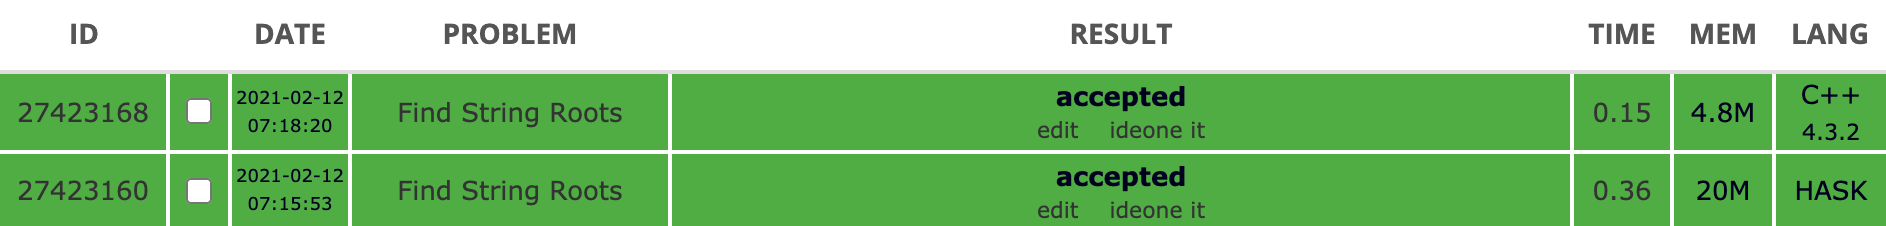
\includegraphics[width=\textwidth]{spoj/FINDSR-accepted-cpp-haskell}
\caption{El código fue aceptado por el juez en Haskell y C++}
\end{figure}

\newpage


\subsection{Ver si una cadena es una rotación cíclica de otra}

\subsubsection{Análisis}
De igual manera, el en \hyperlink{cyclic_rotation}{capítulo 3 el problema 32.4-7} se había hecho el
análisis del problema, y como este problema es resovler exactamente lo mismo se omitirá el análisis
y su complejidad.

\subsubsection{Entrada}
Este tipo de entrada es la más común que se verá en la programación competitiva; ya que la primera
línea será un entero con el número de casos a resolver, después caso consistirá de dos líneas.

Igual que el problema anterior (e igual que en la mayoría de los problemas de este índole) la
entrada será sobre un alfabeto de \texttt{[a-z]} entonces serán representados en ASCII.

\subsubsection{Salida}
Solo se deberá mostrar en la salida estándar \texttt{Si} o \texttt{No} dependiendo si es una
rotación cíclica.

\subsubsection{Ejemplos}
Dado que ambas cadenas son de la misma longitud se hará lo siguiente, $s = qq$ donde $s$ será el
texto y $p$ el patrón. Entonces con el algoritmo dee Knuth-Morris-Pratt se buscará $p$ en $s$.

\begin{itemize}
\item \texttt{abc} es una rotación cíclica de \texttt{cab} porque \texttt{cab} $\mapsto$
\texttt{abc}. Se muestra en la siguiente tabla de manera gráfica la idea.
\begin{table}[h]
\centering
\begin{tabular}{|c|c|c|c|c|c|}
\hline
\texttt{c}                   &  \cellcolor{green}\texttt{a} &  \cellcolor{green}\texttt{b} &
\cellcolor{green} \texttt{c} &  \texttt{a}                  & \texttt{b}                   \\\hline
\end{tabular}
\end{table}

\item Claramente \texttt{abab} no es rotación cíclica de \texttt{aabb}.
\begin{table}[h]
\centering
\begin{tabular}{|c|c|c|c|c|c|c|c|}
\hline
\texttt{a} & \texttt{b} & \texttt{a} &\texttt{b} & \texttt{a} & \texttt{b} & \texttt{a} & \texttt{b} \\\hline
\end{tabular}
\end{table}
\end{itemize}

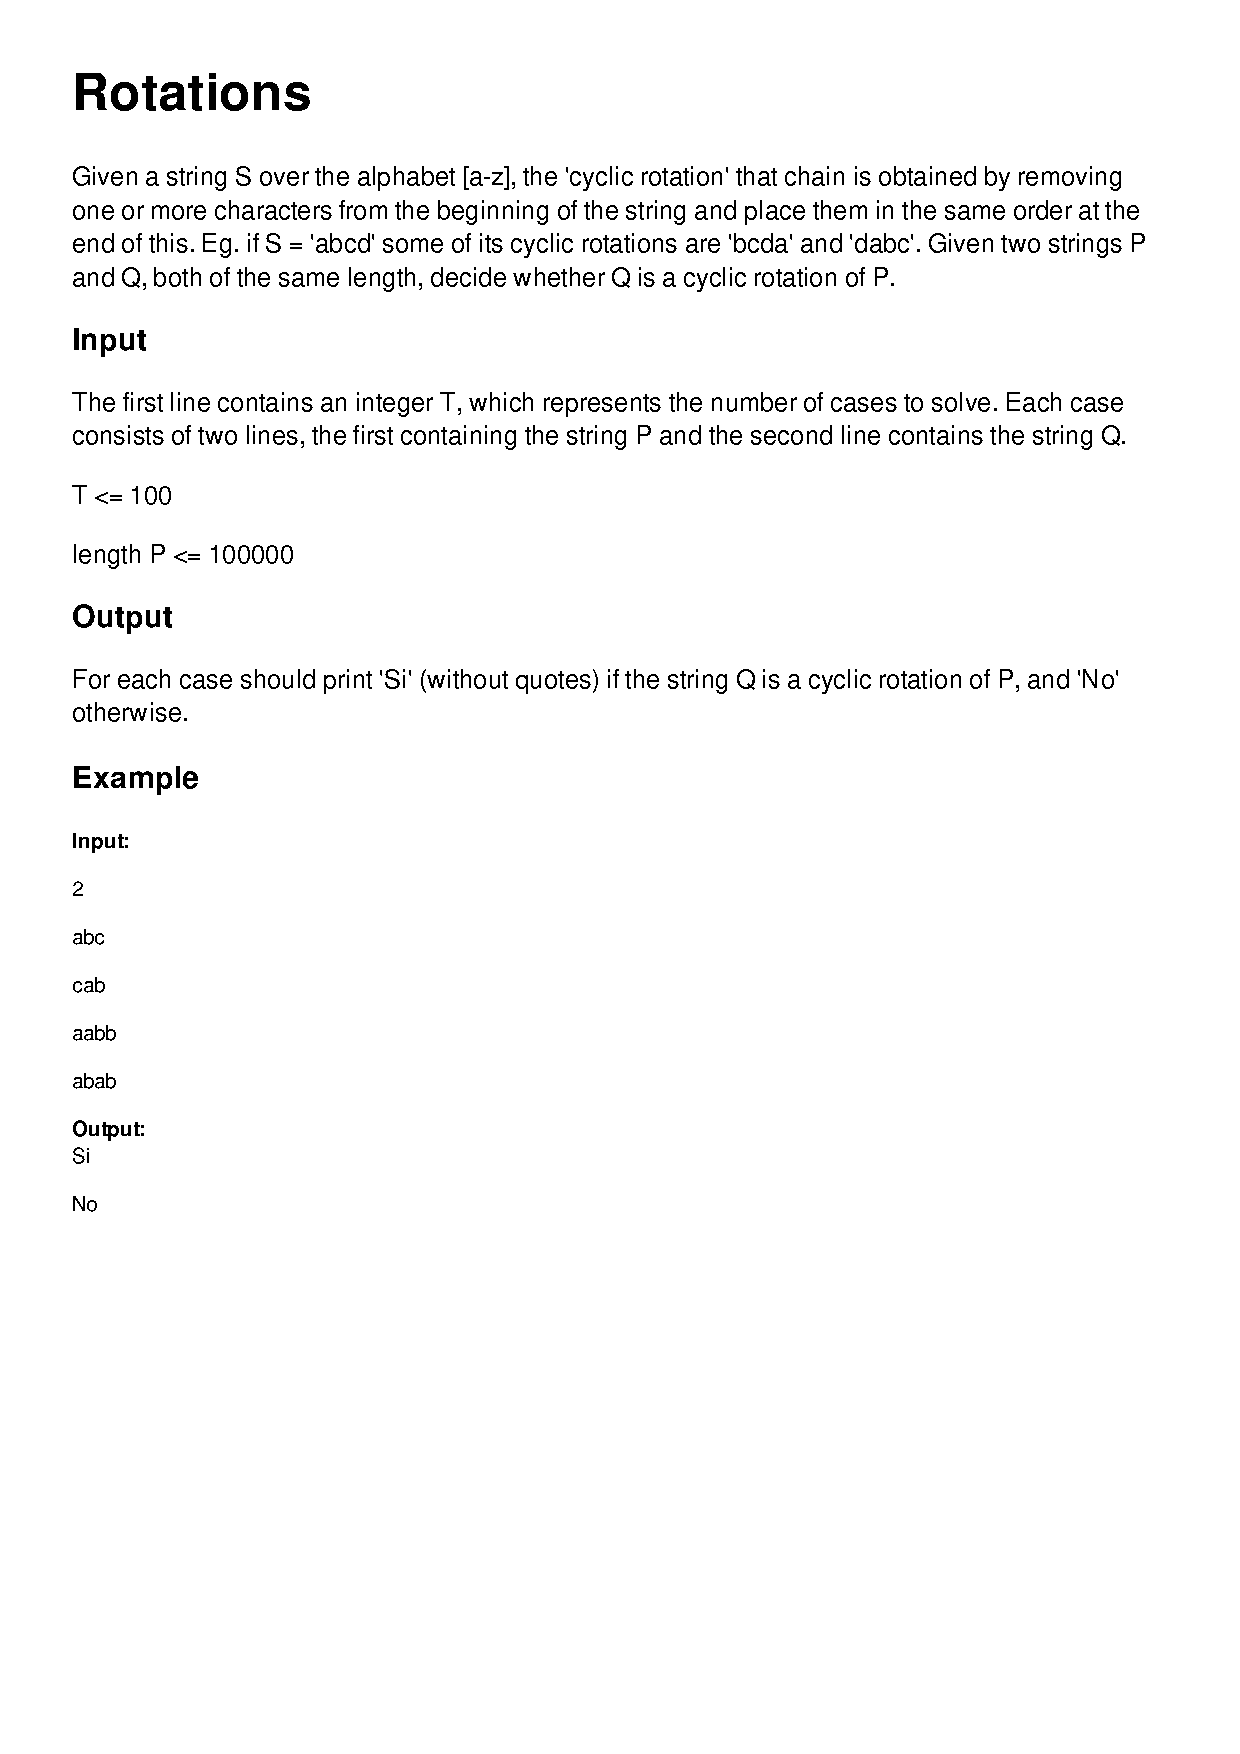
\includepdf[pages=-]{problemas/pdf/EC_WORLD.pdf}

\subsubsection{Implementación en C++}
\inputminted[linenos, frame=lines, fontsize=\footnotesize]{cpp}{problemas/cpp/EC_WORLD.cpp}
\begin{itemize}
\item De línea \texttt{6} a \texttt{19} es la implementación de la función de error.

\item De línea \texttt{21} a \texttt{38} es la implementación del algoritmo Knuth-Morris-Pratt.

\item En línea \texttt{43} se lee el número de casos, y en la \texttt{44} se itera \texttt{t} hasta
que sea 0 y como cualquier valor no cero en \texttt{while} lo toma como falso para la iteración.

\item De la línea \texttt{47} a \texttt{52} es cuando hace la validación dicha en el análisis.

\end{itemize}

\newpage

\subsubsection{Implementación en Haskell}
\inputminted[linenos, frame=lines]{haskell}{problemas/haskell/EC_WORLD.hs}

Muchas veces algunos jueces no aceptan cierto lenguaje, y en este caso el que diseñó el problema y
lo subió en SPOJ, no puso a Haskell para este problema. Pero aún así se hará.

Dado que el tipo de entrada, que es por casos es diferente al problema anterior, la naturaleza de
la entrada y salida será diferente.

\begin{itemize}
\item En la línea \texttt{1} del módulo \hsCode{Control.Monad} se importa la función\\
\hsCode{replicateM :: Applicative m => Int -> m a -> m [a]}, donde\\ \hsCode{replicateM n act}
lleva a cabo una acción $n$ veces, juntando los resultados.

\item De la línea \texttt{4} a \texttt{8} empieza el bloque \hsCode{do} utilizado para las
operaciones de entrada y salida como secuencia.

En la línea \texttt{5} lee una línea, que es el número de casos de la entrada estándar y eso es
transformado con \hsCode{fmap :: (a -> b) -> f a -> f b} a un entero con la función
\hsCode{read :: Read a => String -> a}. Se ocupa el sinónimo infijo \texttt{<\$>} de \hsCode{fmap}.

En la línea \texttt{6} es cuando se lee la entrada de cada caso, primero \hsCode{replicateM t}
ejecuta la acción \hsCode{replicateM 2 getLine} $t$ veces, donde cada una lee de la entrada
estándar 2 veces.

En la línea \texttt{7} como la expresión \hsCode{let} está en el bloque \hsCode{do} se omite el
\hsCode{in} después. Dado que \hsCode{inputs} tiene ligado los valores de la entrada, cada caso que
consiste de una lista de dos elementos es transformado con \texttt{<\$>} por la función
\hsCode{process} que hace el ``algoritmo'' descrito en el análisis.

En la línea \texttt{8} en la función\\
\hsCode{sequence_ :: (Foldable t, Monad m) => t (m a) -> m ()}, que evalúa cada acción monádica de
la estructura plegable de iquierda a derecha e ignora sus resultados, los hacemos porque serán
puras acciones \hsCode{IO ()}, \hsCode{sequence_} recibe como argumento acciones monádicas donde
cada \texttt{answer} se imprime en la salida estándar con \hsCode{putStrLn :: String -> IO ()}. 

\item De la línea \texttt{10} a \texttt{16} es see crea la función
\hsCode{process :: [String] -> String}, donde por medio de caza de patrones se trabaja con una
lista de dos elementos, acto seguido en la expresión \hsCode{let ... in ..} se busca la ocurrencia
del patrón \texttt{p} en \texttt{s} y al final con la función
\hsCode{null :: Foldable t => t a -> Bool} se verifica si la lista es vacía.  

\item De la línea \texttt{19} a \texttt{24} es la implementación del algoritmo Knuth-Morris-Pratt
funcionalmente.
\end{itemize}

\subsubsection{Resultado del juez}
\begin{figure}[H]
\centering
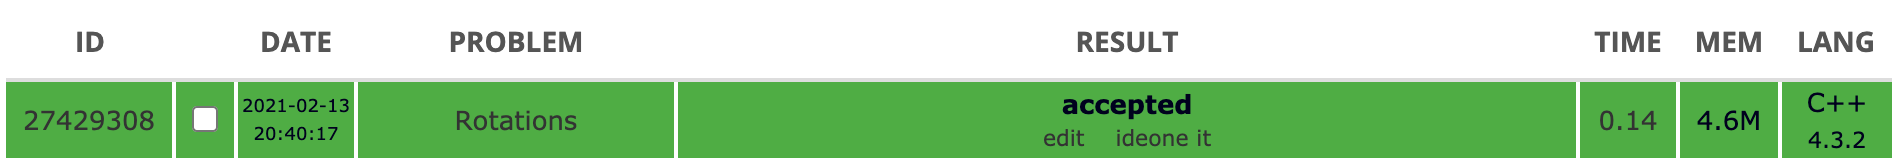
\includegraphics[width=\textwidth]{spoj/EC_WORLD-accepted-cpp}
\caption{El código fue aceptado por el juez en C++}
\end{figure}

\newpage


\subsection{Extender una cadena a un palíndromo}

\subsubsection{Análisis}
En este problema lo \textit{realmente importante} empieza en el tercer párrafo, que resumiendo es:

\begin{tcolorbox}
Dada una cadena, producir el palíndromo\footnote{Un palíndromo es una palabra o frase que se lee
igual en un sentido que en otro. Por ejemplo: arenera, oso, radar, sometemos, etc.} más corto que
puede ser formado agregando cero o más caracteres al final de la cadena.
\end{tcolorbox}

Una forma ingenua de resolver este problema es simplemente concatenando la cadena original $s$
con su reversa $s^R$, i.e., $t = ss^R$ donde $t$ ya es un palíndromo, y a pesar de que resuelve el
problema no se asegura que sea el palíndromo más corto.

Para mostrarlo tomemos una cadena arbitraria $s = $ \texttt{recono} y $s^R =$ \texttt{onocer}
quedando $t = $ \texttt{reconoonocer} y $t$ es un palíndromo pero hay un palíndromo más corto
$t' = $ \texttt{reconocer}. Esto fue concatenando \texttt{cer} a \texttt{recono}. 
Por lo tanto debe de haber una forma mejor de atacar el problema.

Consideremos la función de error utilizada en KMP, como por hipótesis del problema la cadena solo
consiste de letras mayúsculas y minúsculas, se puede usar un tipo de ``separador'' al procesar lo
siguiente; sea $r = s^R$\texttt{\$}$s$ donde $r$ es la concatenación de la reveresa de la cadena de
entrada concatenada con el símbolo \texttt{\$} como separador, y la cadena original.

Entonces se procesará $r$ con la función de error, y ésta indicará el prefijo más largo de $s^R$
que es sufijo de $s$, denominemos a tal la subcadena como $s'$ tal que $s' \sqsubset s^R$ y
$s' \sqsupset s$, esto para saber de antemano la subcadena que se traslapa en $s$ y $s^R$. Para
obtener $s'$ tomemos $n = \vert t \vert$ y $\pi$ la función de error donde $\pi[n] = k$ es la 
longitud de $s'$. Para finalmente tener el palíndromo más pequeño se toma la cadena original $s$
concatenada con $u = s^R[k \ldots]$ donde $u$ es la subcadena de $s^R$ desde $k$.

La complejidad del algoritmo es $\Theta(m)$ donde $m$ es el tamaño de la cadena de entrada tanto
en espacio y tiempo, esto es por construir la función de error y obtener la reversa de una cadena.

\subsubsection{Entrada}
Al igual que el primero problema, la entrada será leída línea por línea hasta EOF yla
entrada será sobre un alfabeto de \texttt{[a-z]|[A-Z]} entonces serán representados en ASCII.

\subsubsection{Salida}
Una sola línea que se imprime en la salida estándar con el palíndromo de más corto.

\subsubsection{Ejemplos}
\begin{itemize}
\item Sea $s = $ \texttt{aaaa}, $s^R =$ \texttt{aaaa} y finalmente
$r = s^R$\texttt{\$}$s =$ \texttt{aaaa\$aaaa} y se construye la función de error con $r$ quedando,

\begin{table}[h]
\centering
\begin{tabular}{c|c|c|c|c|c|c|c|c|c|}
\cline{2-10}
$i$      & 1          & 2          & 3          & 4          & 5           & 6          & 7          & 8          & 9          \\ \hline
$P[i]$   & \texttt{a} & \texttt{a} & \texttt{a} & \texttt{a} & \texttt{\$} & \texttt{a} & \texttt{a} & \texttt{a} & \texttt{a} \\ \hline
$\pi[i]$ & 0          & 1          & 2          & 3          & 0           & 1          & 2          & 3          & 4          \\ \cline{2-10} 
\end{tabular}
\end{table}
Para obtener $s'$ tomemos $n = \vert r \vert = 9$ y en $\pi[9] = 4$ donde $\vert s' \vert = 4$.\\
Siendo el palíndromo más corto como
$u = s \cdot s^R[4 \ldots] =$ \texttt{aaaa}$\cdot \varepsilon$ = \texttt{aaaa}.

\item Sea $s = $ \texttt{abba}, $s^R =$ \texttt{abba} y finalmente
$r = s^R$\texttt{\$}$s =$ \texttt{abba\$abba} y se construye la función de error con $r$ quedando,

\begin{table}[h]
\centering
\begin{tabular}{c|c|c|c|c|c|c|c|c|c|}
\cline{2-10}
$i$      & 1          & 2          & 3          & 4          & 5           & 6          & 7          & 8          & 9          \\ \hline
$P[i]$   & \texttt{a} & \texttt{b} & \texttt{b} & \texttt{a} & \texttt{\$} & \texttt{a} & \texttt{b} & \texttt{b} & \texttt{a} \\ \hline
$\pi[i]$ & 0          & 0          & 0          & 1          & 0           & 1          & 2          & 3          & 4          \\ \cline{2-10} 
\end{tabular}
\end{table}
Para obtener $s'$ tomemos $n = \vert r \vert = 9$ y en $\pi[9] = 4$ donde $\vert s' \vert = 4$.\\
Siendo el palíndromo más corto como
$u = s \cdot s^R[4 \ldots] =$ \texttt{abba}$\cdot \varepsilon$ = \texttt{abba}.

\item Sea $s = $ \texttt{amanaplanacanal}, $s^R =$ \texttt{lanacanalpanama} y finalmente\\
$r = s^R$\texttt{\$}$s =$ \texttt{lanacanalpanama\$amanaplanacanal} y se construye la función de
error con $r$ quedando,

\begin{table}[h]
\centering
\begin{tabular}{c|c|c|c|c|c|c|c|c|c|c|c|c|c|c|c|c|}
\cline{2-17}
$i$      & 1          & 2          & 3          & 4          & 5          & 6          & 7          & 8          & 9          & 10         & 11         & 12         & 13         & 14         & 15         & 16          \\ \hline
$P[i]$   & \texttt{l} & \texttt{a} & \texttt{n} & \texttt{a} & \texttt{c} & \texttt{a} & \texttt{n} & \texttt{a} & \texttt{l} & \texttt{p} & \texttt{a} & \texttt{n} & \texttt{a} & \texttt{m} & \texttt{a} & \texttt{\$} \\ \hline
$\pi[i]$ & 0          & 0          & 0          & 0          & 0          & 0          & 0          & 0          & 1          & 0          & 0          & 0          & 0          & 0          & 0          & 0           \\ \cline{2-17} 
\end{tabular}
\end{table}

\begin{table}[H]
\centering
\begin{tabular}{c|c|c|c|c|c|c|c|c|c|c|c|c|c|c|c|}
\cline{2-16}
$i$      & 17         & 18         & 19         & 20         & 21         & 22         & 23         & 24         & 25         & 26        & 27          & 28         & 29         & 30         & 31          \\ \hline
$P[i]$   & \texttt{a} & \texttt{m} & \texttt{a} & \texttt{n} & \texttt{a} & \texttt{p} & \texttt{l} & \texttt{a} & \texttt{n} & \texttt{a} & \texttt{c} & \texttt{a} & \texttt{n} & \texttt{a} & \texttt{l}  \\ \hline
$\pi[i]$ & 0          & 0          & 0          & 0          & 0          & 0          & 1          & 2          & 3          & 4          & 5          & 6          & 7          & 8          & 9           \\ \cline{2-16} 
\end{tabular}
\end{table}
Para obtener $s'$ tomemos $n = \vert r \vert = 31$ y en $\pi[31] = 9$ donde $\vert s' \vert = 9$.\\
Siendo el palíndromo más corto como $u = s \cdot s^R[9 \ldots] =$\\
\texttt{amanaplanacanal}$\cdot$\texttt{panama} = \texttt{amanaplanacanalpanama}.

\item Sea $s = $ \texttt{xyz}, $s^R =$ \texttt{zyx} y finalmente
$r = s^R$\texttt{\$}$s =$ \texttt{xyz\$zyx} y se construye la función de error con $r$ quedando,

\begin{table}[H]
\centering
\begin{tabular}{c|c|c|c|c|c|c|c|}
\cline{2-8}
$i$      & 1          & 2          & 3          & 4           & 5          & 6          & 7          \\ \hline
$P[i]$   & \texttt{z} & \texttt{y} & \texttt{x} & \texttt{\$} & \texttt{x} & \texttt{y} & \texttt{z} \\ \hline
$\pi[i]$ & 0          & 0          & 0          & 0           & 0          & 0          & 1          \\ \cline{2-8} 
\end{tabular}
\end{table}
Para obtener $s'$ tomemos $n = \vert r \vert = 7$ y en $\pi[7] = 1$ donde $\vert s' \vert = 1$.\\
Siendo el palíndromo más corto como
$u = s \cdot s^R[1 \ldots] =$ \texttt{xyz}$\cdot$\texttt{yx} = \texttt{xyzyx}.

\end{itemize}

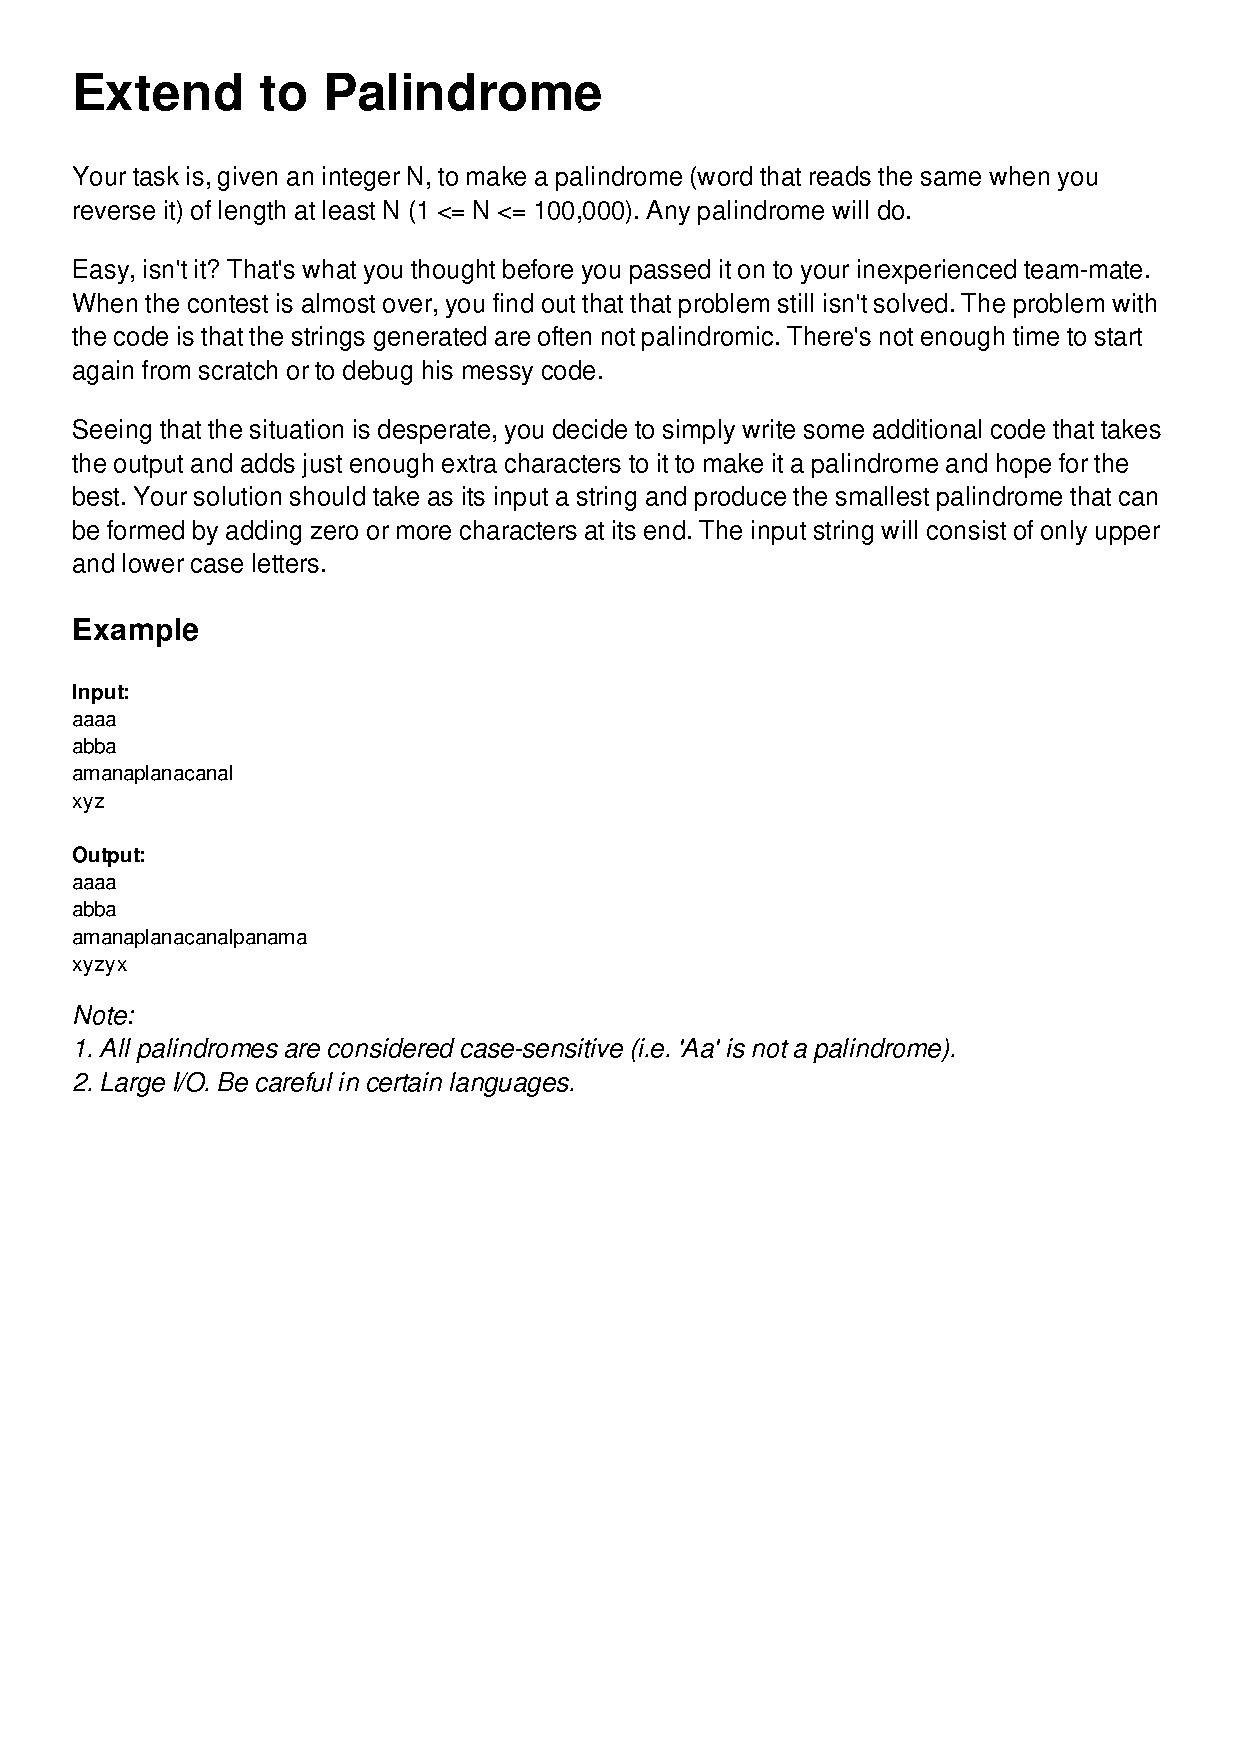
\includepdf[pages=-]{problemas/pdf/EPALIN.pdf}

\subsubsection{Implementación en C++}
\inputminted[linenos, frame=lines]{cpp}{problemas/cpp/EPALIN.cpp}

\begin{itemize}
\item En la línea \texttt{24} se hace una copia de la línea que se leyó
\item En la línea \texttt{26} se crea la cadena $r$.
\item En la línea \texttt{31, 32} se acompleta la cadena original para que sea un palíndromo.
\end{itemize}

\subsubsection{Implementación en Haskell}
\inputminted[linenos, frame=lines]{haskell}{problemas/haskell/EPALIN.hs}

\begin{itemize}
\item Al igual que el primer problema, se tratará la entrada y salida orientada a líneas con
la función \hsCode{interact} donde la función \hsCode{process} es la que hará \textit{el algorítmo}.
\item En la línea \texttt{8} se saca la reversa de la cadena de entrada, en la línea \texttt{9}
se crea la cadena $r$, en la línea \texttt{10} se crea la función de error. Finalmente en la línea
\texttt{13} con la \hsCode{drop :: Int -> [a] -> [a]} que regresa el sufijo de una lista
\texttt{xs} después de los primeros $n$ elementos, se obtiene la cadena faltante para completar el
palíndromo y en la línea \texttt{14} se concatena \texttt{xs} la cadena anterior.
\end{itemize}

\subsubsection{Resultado del juez}
\begin{figure}[H]
\centering
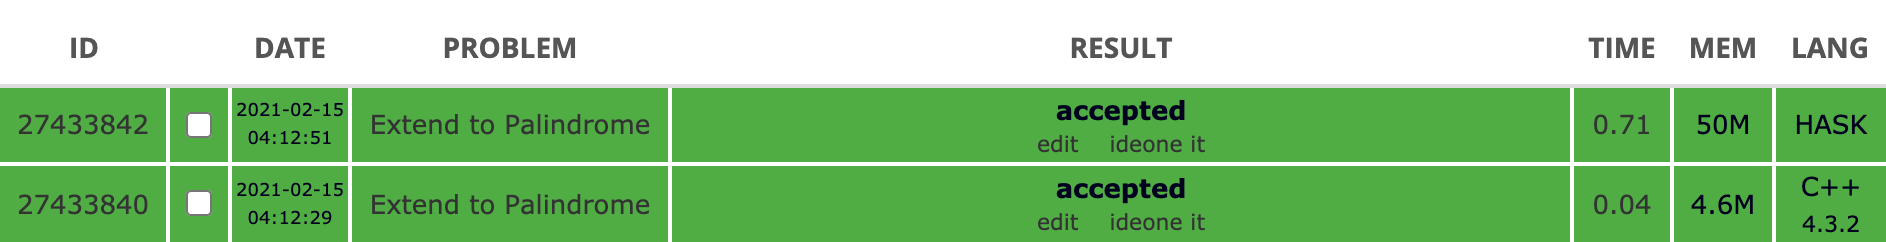
\includegraphics[width=\textwidth]{spoj/EPALIN-accepted-cpp-haskell}
\caption{El código fue aceptado por el juez en Haskell y C++}
\end{figure}

\newpage


\subsection{Encontrar todas las ocurrencias de un patrón en un texto}

\subsubsection{Análisis}
De los problemas anteriores este es quizás es el uso más \textit{canónico} del algoritmo
Knuth-Morris-Pratt per se, ya que solo se pide encontrar todas las posiciones 0-indexadas de
un patrón en un texto. Lo inlcuí porque ``la trampa'' de este problema es que mucha gente lo
resuelve con el algoritmo \textit{naïve} y simplemente el juez no lo aceptará. La complejidad como
ya se había comentado enteriormente, es $\Theta(m)$ en tiempo el preprocesamiento del patrón y
$\Theta(n)$ en encontrar las ocurrencias, en espacio toma complejidad $O(m)$.
%TODO: poner que está chido porque se pueden encontrar patrones que se overlapean

\subsubsection{Entrada}
Al igual que el primer problemas se leerá hasta EOF, y cada caso prueba consistirá de 3 líneas;
la primera será la longitud del patrón, seguida del patrón y después el texo.

\subsubsection{Salida}
Si hubo una(s) aparición(es) cada una será impresa en pantalla línea por línea. Si no, solamente
se imprirá un salto de línea.

\subsubsection{Ejemplos}
\begin{itemize}
\item El patón es \texttt{na} y el texto es \texttt{banananobano}, y hubo 2 apariciones del patrón
en las posiciones 2 y 4.
\begin{table}[h]
\centering
\begin{tabular}{|c|c|
>{\columncolor[HTML]{F5B7B1}}c|
>{\columncolor[HTML]{F5B7B1}}c|
>{\columncolor[HTML]{D7BDE2}}c|
>{\columncolor[HTML]{D7BDE2}}c|c|c|c|c|c|c|}
\hline
\texttt{b} & \texttt{a} & \texttt{n} & \texttt{a} & \texttt{n} & \texttt{a} & \texttt{n} &
\texttt{o} & \texttt{b} & \texttt{a} & \texttt{n} & \texttt{o} \\ \hline
\end{tabular}
\end{table}

\item El patón es \texttt{foobar} y el texto es \texttt{foo}, y no hubo ninguna aparición del
patrón.
\begin{table}[H]
\centering
\begin{tabular}{|c|c|c|}
\hline
\texttt{f} & \texttt{o} & \texttt{o} \\ \hline
\end{tabular}
\end{table}

\item El patón es \texttt{foobarfoo} y el texto es \texttt{barfoobarfoobarfoobarfoobarfoo}, y
hubo 4 apariciones del patrónen la posiciones 3, 9, 15 y 21.
\begin{table}[H]
\centering
\hspace*{-3cm}
\footnotesize
\begin{tabular}{|c|c|c|
>{\columncolor[HTML]{AED6F1}}c|
>{\columncolor[HTML]{AED6F1}}c|
>{\columncolor[HTML]{AED6F1}}c|
>{\columncolor[HTML]{AED6F1}}c|
>{\columncolor[HTML]{AED6F1}}c|
>{\columncolor[HTML]{AED6F1}}c|
>{\columncolor[HTML]{AED6F1}}c|
>{\columncolor[HTML]{AED6F1}}c|
>{\columncolor[HTML]{AED6F1}}c|c|c|c|c|c|c|c|c|c|c|c|c|c|c|c|c|c|c|c|}
\hline
\texttt{b} & \texttt{a} & \texttt{r} & \texttt{f} & \texttt{o} & \texttt{o} & \texttt{b} &
\texttt{a} & \texttt{r} & \texttt{f} & \texttt{o} & \texttt{o} & \texttt{b} & \texttt{a} &
\texttt{r} & \texttt{f} & \texttt{o} & \texttt{o} & \texttt{b} & \texttt{a} & \texttt{r} &
\texttt{f} & \texttt{o} & \texttt{o} & \texttt{b} & \texttt{a} & \texttt{r} & \texttt{f} &
\texttt{o} & \texttt{o} \\ \hline
\end{tabular}
\end{table}

\begin{table}[H]
\centering
\hspace*{-3cm}
\footnotesize
\begin{tabular}{|c|c|c|c|c|c|c|c|c|
>{\columncolor[HTML]{ABEBC6}}c|
>{\columncolor[HTML]{ABEBC6}}c|
>{\columncolor[HTML]{ABEBC6}}c|
>{\columncolor[HTML]{ABEBC6}}c|
>{\columncolor[HTML]{ABEBC6}}c|
>{\columncolor[HTML]{ABEBC6}}c|
>{\columncolor[HTML]{ABEBC6}}c|
>{\columncolor[HTML]{ABEBC6}}c|
>{\columncolor[HTML]{ABEBC6}}c|c|c|c|c|c|c|c|c|c|c|c|c|c|}
\hline
\texttt{b} & \texttt{a} & \texttt{r} & \texttt{f} & \texttt{o} & \texttt{o} & \texttt{b} &
\texttt{a} & \texttt{r} & \texttt{f} & \texttt{o} & \texttt{o} & \texttt{b} & \texttt{a} &
\texttt{r} & \texttt{f} & \texttt{o} & \texttt{o} & \texttt{b} & \texttt{a} & \texttt{r} &
\texttt{f} & \texttt{o} & \texttt{o} & \texttt{b} & \texttt{a} & \texttt{r} & \texttt{f} &
\texttt{o} & \texttt{o} \\ \hline
\end{tabular}
\end{table}

\begin{table}[H]
\centering
\hspace*{-3cm}
\footnotesize
\begin{tabular}{|c|c|c|c|c|c|c|c|c|c|c|c|c|c|c|
>{\columncolor[HTML]{F9E79F}}c|
>{\columncolor[HTML]{F9E79F}}c|
>{\columncolor[HTML]{F9E79F}}c|
>{\columncolor[HTML]{F9E79F}}c|
>{\columncolor[HTML]{F9E79F}}c|
>{\columncolor[HTML]{F9E79F}}c|
>{\columncolor[HTML]{F9E79F}}c|
>{\columncolor[HTML]{F9E79F}}c|
>{\columncolor[HTML]{F9E79F}}c|c|c|c|c|c|c|c|}
\hline
\texttt{b} & \texttt{a} & \texttt{r} & \texttt{f} & \texttt{o} & \texttt{o} & \texttt{b} &
\texttt{a} & \texttt{r} & \texttt{f} & \texttt{o} & \texttt{o} & \texttt{b} & \texttt{a} &
\texttt{r} & \texttt{f} & \texttt{o} & \texttt{o} & \texttt{b} & \texttt{a} & \texttt{r} &
\texttt{f} & \texttt{o} & \texttt{o} & \texttt{b} & \texttt{a} & \texttt{r} & \texttt{f} &
\texttt{o} & \texttt{o} \\ \hline
\end{tabular}
\end{table}

\begin{table}[H]
\centering
\hspace*{-3cm}
\footnotesize
\begin{tabular}{|c|c|c|c|c|c|c|c|c|c|c|c|c|c|c|c|c|c|c|c|c|
>{\columncolor[HTML]{EDBB99}}c|
>{\columncolor[HTML]{EDBB99}}c|
>{\columncolor[HTML]{EDBB99}}c|
>{\columncolor[HTML]{EDBB99}}c|
>{\columncolor[HTML]{EDBB99}}c|
>{\columncolor[HTML]{EDBB99}}c|
>{\columncolor[HTML]{EDBB99}}c|
>{\columncolor[HTML]{EDBB99}}c|
>{\columncolor[HTML]{EDBB99}}c|c|}
\hline
\texttt{b} & \texttt{a} & \texttt{r} & \texttt{f} & \texttt{o} & \texttt{o} & \texttt{b} &
\texttt{a} & \texttt{r} & \texttt{f} & \texttt{o} & \texttt{o} & \texttt{b} & \texttt{a} &
\texttt{r} & \texttt{f} & \texttt{o} & \texttt{o} & \texttt{b} & \texttt{a} & \texttt{r} &
\texttt{f} & \texttt{o} & \texttt{o} & \texttt{b} & \texttt{a} & \texttt{r} & \texttt{f} &
\texttt{o} & \texttt{o} \\ \hline
\end{tabular}
\end{table}

\end{itemize}

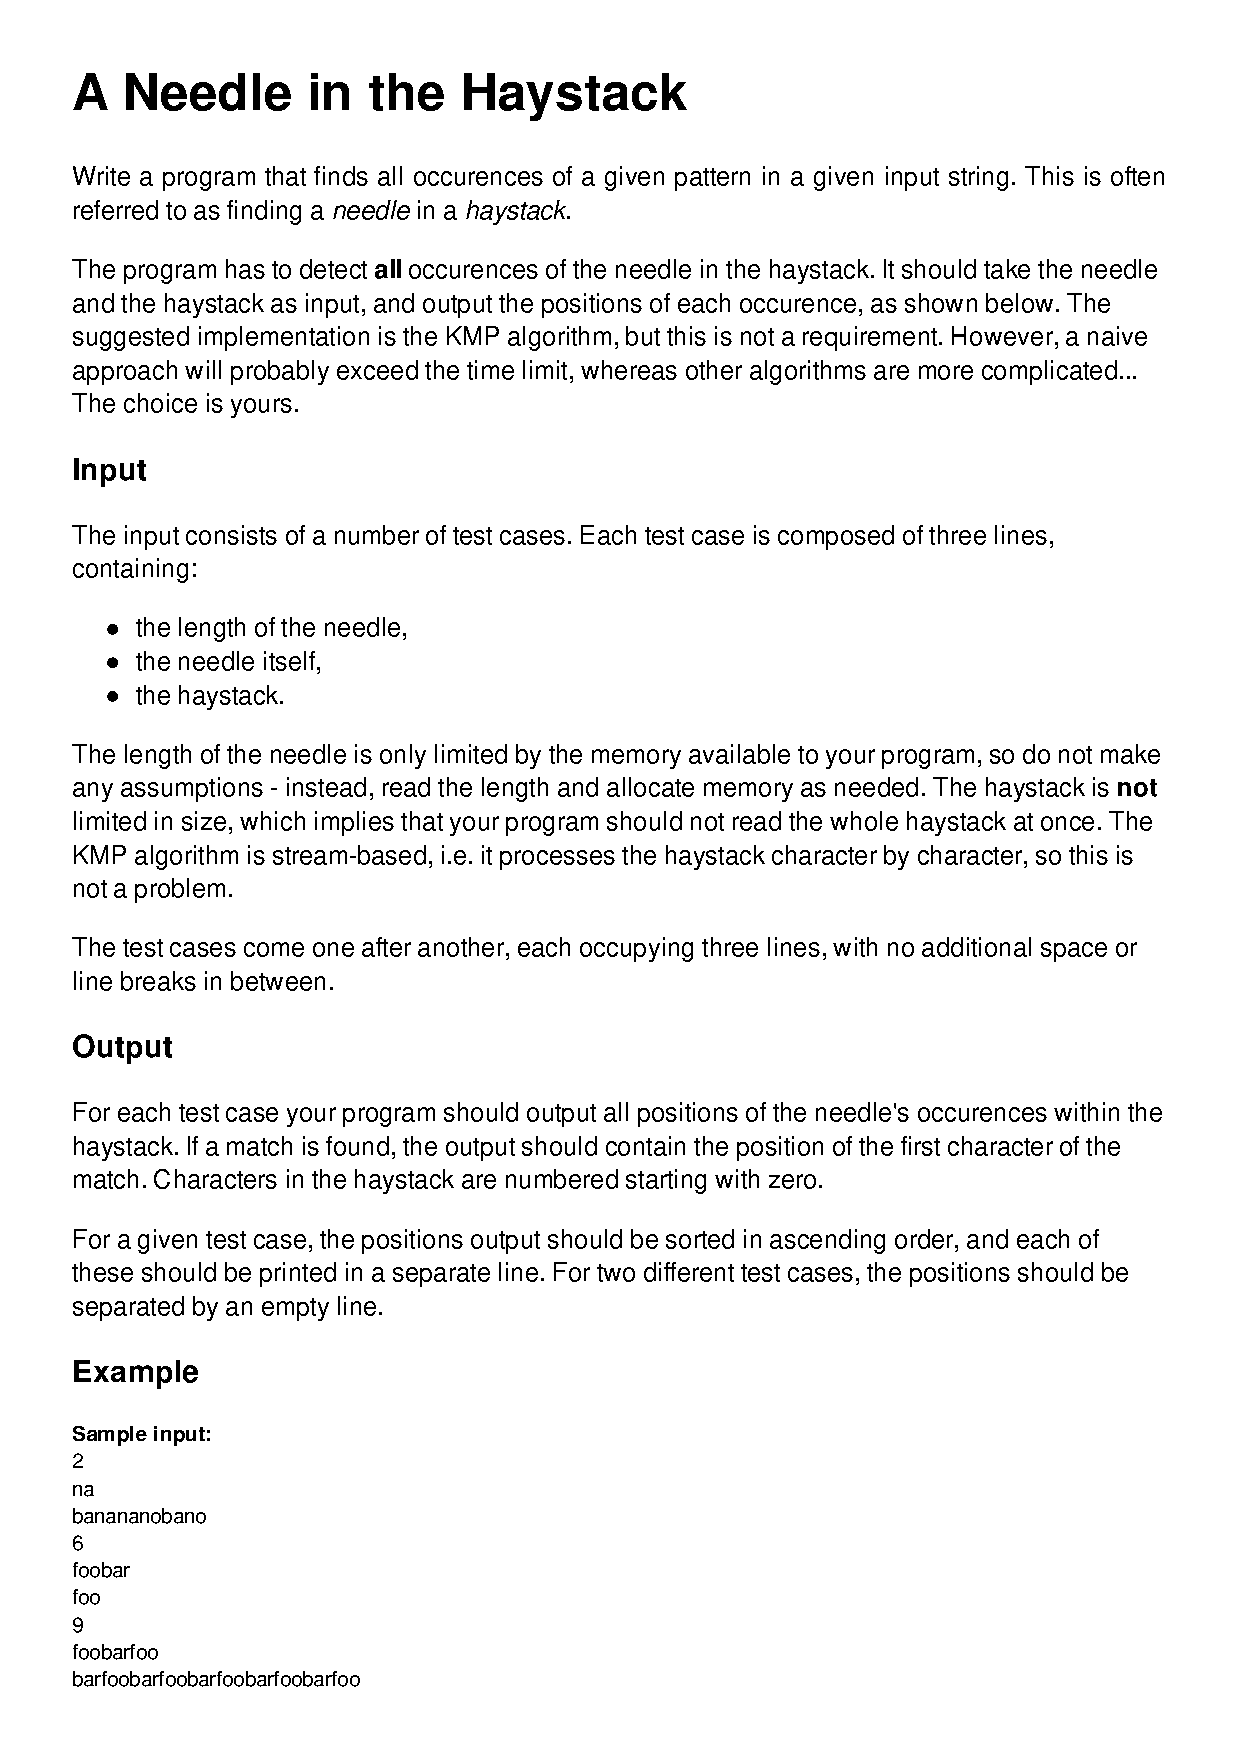
\includepdf[pages=-]{problemas/pdf/NHAY.pdf}

\subsubsection{Implementación en C++}
\inputminted[linenos, frame=lines, fontsize=\footnotesize]{cpp}{problemas/cpp/NHAY.cpp}

\subsubsection{Implementación en Haskell}
\inputminted[linenos, frame=lines]{haskell}{problemas/haskell/NHAY.hs}

\begin{itemize}
\item Al ser un programa orientado a líneas, solo se prestará atención a la función
\hsCode{process} y \hsCode{parse}.

En la función \hsCode{parse} se usa para \textit{procesar} de tres en tres líneas y cada caso
prueba verlo como una sola tupla. En la función \hsCode{process} en la línea \texttt{12} busca
las apariciones del patrón en el texto, seguido en la línea \texttt{14} verifica si es una lista
vacía, si lo es solamente regresa un salto de línea, si no con la función
\hsCode{intercalate :: [a] -> [[a]] -> [a]} que inserta el primer argumento entre cada elemento
de la lista y concatena el resultado, pone un salto de línea entre cada índice de cada ocurrencia.
\end{itemize}

\subsubsection{Resultado del juez}
\begin{figure}[h]
\centering
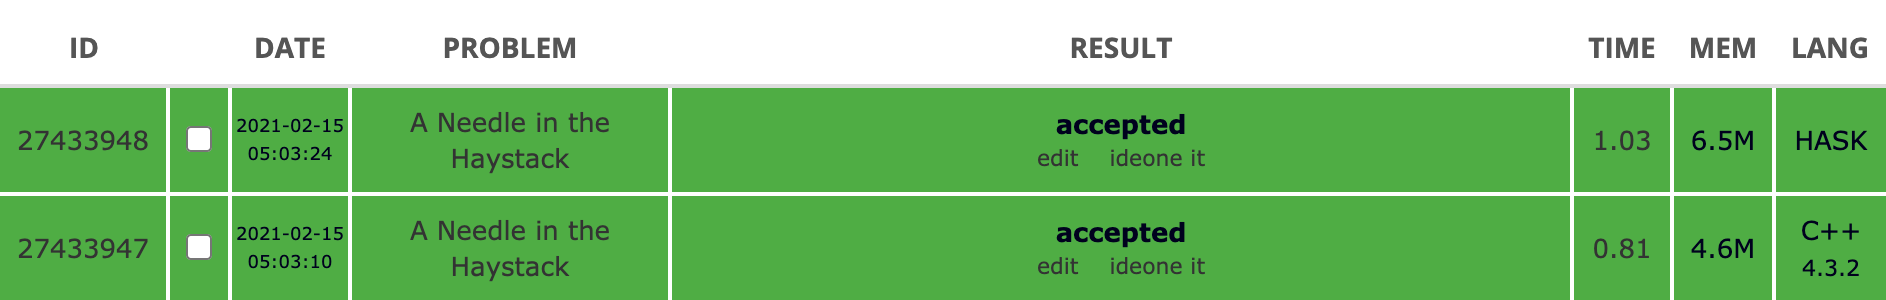
\includegraphics[width=\textwidth]{spoj/NHAY-accepted-cpp-haskell}
\caption{El código fue aceptado por el juez en Haskell y C++}
\end{figure}

% TODO: poner que puedo optimizar la entrada con Data.ByteString.Char8
    
    \chapter{Conclusiones}
        \input{capitulos/conclusiones}
    
    \begin{appendices}
        %Para darle formato al código en Haskell (dado que hacerlo de forma manual) es una tanto tedioso se utilizó
%\href{https://github.com/jaspervdj/stylish-haskell}{\texttt{stylish-haskell}}.

%A la hora de buscar ``símbolos'' en de manera más inteligente en \LaTeX se utilizó
%\href{https://github.com/jaspervdj/stylish-haskell}{Detexify}, haciendo un ezbozo del símbolo
%a buscar y nos dará sugerencias de cuál podría ser.


%De igual manera el código en C++ se le dio estiló uttilizando el estándar de \href{https://llvm.org/docs/CodingStandards.html}{LLVM}

%Lazy I/O

%# Explicar la entrada en haskell

%Ver si cambio `fmap` con `<$>`

%- `lines`,
%- Para leer cada test case use una función auxiliar llamada `join`

\section{Compilar y ejecutar código}

        
        % TODO: poner que así organizo los .bib
% https://flamingtempura.github.io/bibtex-tidy/            
    \end{appendices}

\backmatter
    \nocite{*}
    \printbibliography

\end{document}
